\documentclass[a4paper]{book}
\usepackage{a4wide}
\usepackage{makeidx}
\usepackage{graphicx}
\usepackage{multicol}
\usepackage{float}
\usepackage{listings}
\usepackage{color}
\usepackage{textcomp}
\usepackage{alltt}
\usepackage{times}
\usepackage{ifpdf}
\ifpdf
\usepackage[pdftex,
            pagebackref=true,
            colorlinks=true,
            linkcolor=blue,
            unicode
           ]{hyperref}
\else
\usepackage[ps2pdf,
            pagebackref=true,
            colorlinks=true,
            linkcolor=blue,
            unicode
           ]{hyperref}
\usepackage{pspicture}
\fi
\usepackage[utf8]{inputenc}
\usepackage{doxygen}
\lstset{language=C++,inputencoding=utf8,basicstyle=\footnotesize,breaklines=true,breakatwhitespace=true,tabsize=8,numbers=left }
\makeindex
\setcounter{tocdepth}{3}
\renewcommand{\footrulewidth}{0.4pt}
\begin{document}
\hypersetup{pageanchor=false}
\begin{titlepage}
\vspace*{7cm}
\begin{center}
{\Large Hamilton College CS110 Graphics Library \\[1ex]\large 1.0 }\\
\vspace*{1cm}
{\large Generated by Doxygen 1.6.1}\\
\vspace*{0.5cm}
{\small Fri Jul 7 13:57:20 2017}\\
\end{center}
\end{titlepage}
\clearemptydoublepage
\pagenumbering{roman}
\tableofcontents
\clearemptydoublepage
\pagenumbering{arabic}
\hypersetup{pageanchor=true}
\chapter{Namespace Index}
\section{Package List}
Here are the packages with brief descriptions (if available):\begin{DoxyCompactList}
\item\contentsline{section}{\hyperlink{namespacecs110graphics}{cs110graphics} (Contains a CSPy-\/friendly version of a Tkinter based graphics library )}{\pageref{namespacecs110graphics}}{}
\end{DoxyCompactList}

\chapter{Class Index}
\section{Class Hierarchy}
This inheritance list is sorted roughly, but not completely, alphabetically:\begin{DoxyCompactList}
\item \contentsline{section}{cs110graphics.\_\-RunWithYieldDelay}{\pageref{classcs110graphics_1_1__RunWithYieldDelay}}{}
\item \contentsline{section}{cs110graphics.Event}{\pageref{classcs110graphics_1_1Event}}{}
\item \contentsline{section}{cs110graphics.EventHandler}{\pageref{classcs110graphics_1_1EventHandler}}{}
\item \contentsline{section}{cs110graphics.GraphicalObject}{\pageref{classcs110graphics_1_1GraphicalObject}}{}
\begin{DoxyCompactList}
\item \contentsline{section}{cs110graphics.Fillable}{\pageref{classcs110graphics_1_1Fillable}}{}
\begin{DoxyCompactList}
\item \contentsline{section}{cs110graphics.Circle}{\pageref{classcs110graphics_1_1Circle}}{}
\item \contentsline{section}{cs110graphics.Oval}{\pageref{classcs110graphics_1_1Oval}}{}
\item \contentsline{section}{cs110graphics.Polygon}{\pageref{classcs110graphics_1_1Polygon}}{}
\item \contentsline{section}{cs110graphics.Rectangle}{\pageref{classcs110graphics_1_1Rectangle}}{}
\item \contentsline{section}{cs110graphics.Square}{\pageref{classcs110graphics_1_1Square}}{}
\end{DoxyCompactList}
\item \contentsline{section}{cs110graphics.Image}{\pageref{classcs110graphics_1_1Image}}{}
\item \contentsline{section}{cs110graphics.Text}{\pageref{classcs110graphics_1_1Text}}{}
\end{DoxyCompactList}
\item \contentsline{section}{cs110graphics.Timer}{\pageref{classcs110graphics_1_1Timer}}{}
\item \contentsline{section}{cs110graphics.Window}{\pageref{classcs110graphics_1_1Window}}{}
\end{DoxyCompactList}

\chapter{Class Index}
\section{Class List}
Here are the classes, structs, unions and interfaces with brief descriptions:\begin{DoxyCompactList}
\item\contentsline{section}{\hyperlink{classcs110graphics_1_1__RunWithYieldDelay}{cs110graphics.\_\-RunWithYieldDelay} (A class which uses a function which returns a generator to rerun until the generator stops generating numbers )}{\pageref{classcs110graphics_1_1__RunWithYieldDelay}}{}
\item\contentsline{section}{\hyperlink{classcs110graphics_1_1Circle}{cs110graphics.Circle} (A circle, which can be added to a \hyperlink{classcs110graphics_1_1Window}{Window} object )}{\pageref{classcs110graphics_1_1Circle}}{}
\item\contentsline{section}{\hyperlink{classcs110graphics_1_1Event}{cs110graphics.Event} (An event which gets bound to an object )}{\pageref{classcs110graphics_1_1Event}}{}
\item\contentsline{section}{\hyperlink{classcs110graphics_1_1EventHandler}{cs110graphics.EventHandler} (Handles an event )}{\pageref{classcs110graphics_1_1EventHandler}}{}
\item\contentsline{section}{\hyperlink{classcs110graphics_1_1Fillable}{cs110graphics.Fillable} (This window is a parent class of any object which can have its colors modified )}{\pageref{classcs110graphics_1_1Fillable}}{}
\item\contentsline{section}{\hyperlink{classcs110graphics_1_1GraphicalObject}{cs110graphics.GraphicalObject} (This window is a parent class of any object which can be put into \hyperlink{classcs110graphics_1_1Window}{Window} )}{\pageref{classcs110graphics_1_1GraphicalObject}}{}
\item\contentsline{section}{\hyperlink{classcs110graphics_1_1Image}{cs110graphics.Image} (An image, which can be added to a \hyperlink{classcs110graphics_1_1Window}{Window} object )}{\pageref{classcs110graphics_1_1Image}}{}
\item\contentsline{section}{\hyperlink{classcs110graphics_1_1Oval}{cs110graphics.Oval} (An oval, which can be added to a \hyperlink{classcs110graphics_1_1Window}{Window} object )}{\pageref{classcs110graphics_1_1Oval}}{}
\item\contentsline{section}{\hyperlink{classcs110graphics_1_1Polygon}{cs110graphics.Polygon} (A \hyperlink{classcs110graphics_1_1Polygon}{Polygon}, which can be added to a \hyperlink{classcs110graphics_1_1Window}{Window} object )}{\pageref{classcs110graphics_1_1Polygon}}{}
\item\contentsline{section}{\hyperlink{classcs110graphics_1_1Rectangle}{cs110graphics.Rectangle} (A rectangle, which can be added to a \hyperlink{classcs110graphics_1_1Window}{Window} object )}{\pageref{classcs110graphics_1_1Rectangle}}{}
\item\contentsline{section}{\hyperlink{classcs110graphics_1_1Square}{cs110graphics.Square} (A square, which can be added to a \hyperlink{classcs110graphics_1_1Window}{Window} object )}{\pageref{classcs110graphics_1_1Square}}{}
\item\contentsline{section}{\hyperlink{classcs110graphics_1_1Text}{cs110graphics.Text} (\hyperlink{classcs110graphics_1_1Text}{Text} which can be added to a \hyperlink{classcs110graphics_1_1Window}{Window} object )}{\pageref{classcs110graphics_1_1Text}}{}
\item\contentsline{section}{\hyperlink{classcs110graphics_1_1Timer}{cs110graphics.Timer} (A class which continually runs a function after a delay )}{\pageref{classcs110graphics_1_1Timer}}{}
\item\contentsline{section}{\hyperlink{classcs110graphics_1_1Window}{cs110graphics.Window} (This window acts as a canvas which other objects can be put onto )}{\pageref{classcs110graphics_1_1Window}}{}
\end{DoxyCompactList}

\chapter{Namespace Documentation}
\hypertarget{namespacecs110graphics}{
\section{Package cs110graphics}
\label{namespacecs110graphics}\index{cs110graphics@{cs110graphics}}
}


Contains a CSPy-\/friendly version of a Tkinter based graphics library.  
\subsection*{Classes}
\begin{DoxyCompactItemize}
\item 
class \hyperlink{classcs110graphics_1_1Window}{Window}
\begin{DoxyCompactList}\small\item\em This window acts as a canvas which other objects can be put onto. \item\end{DoxyCompactList}\item 
class \hyperlink{classcs110graphics_1_1Event}{Event}
\begin{DoxyCompactList}\small\item\em An event which gets bound to an object. \item\end{DoxyCompactList}\item 
class \hyperlink{classcs110graphics_1_1EventHandler}{EventHandler}
\begin{DoxyCompactList}\small\item\em Handles an event. \item\end{DoxyCompactList}\item 
class \hyperlink{classcs110graphics_1_1GraphicalObject}{GraphicalObject}
\begin{DoxyCompactList}\small\item\em This window is a parent class of any object which can be put into \hyperlink{classcs110graphics_1_1Window}{Window}. \item\end{DoxyCompactList}\item 
class \hyperlink{classcs110graphics_1_1Fillable}{Fillable}
\begin{DoxyCompactList}\small\item\em This window is a parent class of any object which can have its colors modified. \item\end{DoxyCompactList}\item 
class \hyperlink{classcs110graphics_1_1Image}{Image}
\begin{DoxyCompactList}\small\item\em An image, which can be added to a \hyperlink{classcs110graphics_1_1Window}{Window} object. \item\end{DoxyCompactList}\item 
class \hyperlink{classcs110graphics_1_1Text}{Text}
\begin{DoxyCompactList}\small\item\em \hyperlink{classcs110graphics_1_1Text}{Text} which can be added to a \hyperlink{classcs110graphics_1_1Window}{Window} object. \item\end{DoxyCompactList}\item 
class \hyperlink{classcs110graphics_1_1Polygon}{Polygon}
\begin{DoxyCompactList}\small\item\em A \hyperlink{classcs110graphics_1_1Polygon}{Polygon}, which can be added to a \hyperlink{classcs110graphics_1_1Window}{Window} object. \item\end{DoxyCompactList}\item 
class \hyperlink{classcs110graphics_1_1Circle}{Circle}
\begin{DoxyCompactList}\small\item\em A circle, which can be added to a \hyperlink{classcs110graphics_1_1Window}{Window} object. \item\end{DoxyCompactList}\item 
class \hyperlink{classcs110graphics_1_1Oval}{Oval}
\begin{DoxyCompactList}\small\item\em An oval, which can be added to a \hyperlink{classcs110graphics_1_1Window}{Window} object. \item\end{DoxyCompactList}\item 
class \hyperlink{classcs110graphics_1_1Square}{Square}
\begin{DoxyCompactList}\small\item\em A square, which can be added to a \hyperlink{classcs110graphics_1_1Window}{Window} object. \item\end{DoxyCompactList}\item 
class \hyperlink{classcs110graphics_1_1Rectangle}{Rectangle}
\begin{DoxyCompactList}\small\item\em A rectangle, which can be added to a \hyperlink{classcs110graphics_1_1Window}{Window} object. \item\end{DoxyCompactList}\item 
class \hyperlink{classcs110graphics_1_1Timer}{Timer}
\begin{DoxyCompactList}\small\item\em A class which continually runs a function after a delay. \item\end{DoxyCompactList}\item 
class \hyperlink{classcs110graphics_1_1__RunWithYieldDelay}{\_\-RunWithYieldDelay}
\begin{DoxyCompactList}\small\item\em A class which uses a function which returns a generator to rerun until the generator stops generating numbers. \item\end{DoxyCompactList}\end{DoxyCompactItemize}
\subsection*{Functions}
\begin{DoxyCompactItemize}
\item 
def \hyperlink{namespacecs110graphics_af1a7cabc9d0dea87259e97ad88ef85ac}{StartGraphicsSystem}
\begin{DoxyCompactList}\small\item\em This initalizes the graphics system. \item\end{DoxyCompactList}\item 
def \hyperlink{namespacecs110graphics_a0715c42bb0e296007b96bd0a20903d16}{RunWithYieldDelay}
\begin{DoxyCompactList}\small\item\em A wrapper for the \hyperlink{classcs110graphics_1_1__RunWithYieldDelay}{\_\-RunWithYieldDelay} class. \item\end{DoxyCompactList}\end{DoxyCompactItemize}


\subsection{Detailed Description}
Contains a CSPy-\/friendly version of a Tkinter based graphics library. Paul Magnus '18, Ines Ayara '20, Matthew R. Jenkins '20

Summer 2017 

\subsection{Function Documentation}
\hypertarget{namespacecs110graphics_a0715c42bb0e296007b96bd0a20903d16}{
\index{cs110graphics@{cs110graphics}!RunWithYieldDelay@{RunWithYieldDelay}}
\index{RunWithYieldDelay@{RunWithYieldDelay}!cs110graphics@{cs110graphics}}
\subsubsection[{RunWithYieldDelay}]{\setlength{\rightskip}{0pt plus 5cm}def cs110graphics.RunWithYieldDelay ( {\em window}, \/   {\em func})}}
\label{namespacecs110graphics_a0715c42bb0e296007b96bd0a20903d16}


A wrapper for the \hyperlink{classcs110graphics_1_1__RunWithYieldDelay}{\_\-RunWithYieldDelay} class. THIS SHOULD BE USED INSTEAD OF CREATING AN \hyperlink{classcs110graphics_1_1__RunWithYieldDelay}{\_\-RunWithYieldDelay} INSTANCE.

Required Parameters:
\begin{DoxyItemize}
\item window -\/ \hyperlink{classcs110graphics_1_1Window}{Window}
\item func -\/ function which returns a generator of int 
\end{DoxyItemize}\hypertarget{namespacecs110graphics_af1a7cabc9d0dea87259e97ad88ef85ac}{
\index{cs110graphics@{cs110graphics}!StartGraphicsSystem@{StartGraphicsSystem}}
\index{StartGraphicsSystem@{StartGraphicsSystem}!cs110graphics@{cs110graphics}}
\subsubsection[{StartGraphicsSystem}]{\setlength{\rightskip}{0pt plus 5cm}def cs110graphics.StartGraphicsSystem ( {\em first\_\-function}, \/   {\em width} = {\ttfamily 400}, \/   {\em height} = {\ttfamily 400}, \/   {\em background} = {\ttfamily \char`\"{}white\char`\"{}}, \/   {\em name} = {\ttfamily \char`\"{}Graphics~Window\char`\"{}})}}
\label{namespacecs110graphics_af1a7cabc9d0dea87259e97ad88ef85ac}


This initalizes the graphics system. Required Parameters:
\begin{DoxyItemize}
\item first\_\-function -\/ func
\end{DoxyItemize}

Optional Parameters:
\begin{DoxyItemize}
\item width -\/ int
\item height -\/ int
\item background -\/ string
\item name -\/ string 
\end{DoxyItemize}
\chapter{Class Documentation}
\hypertarget{classcs110graphics_1_1__RunWithYieldDelay}{
\section{cs110graphics.\_\-RunWithYieldDelay Class Reference}
\label{classcs110graphics_1_1__RunWithYieldDelay}\index{cs110graphics::\_\-RunWithYieldDelay@{cs110graphics::\_\-RunWithYieldDelay}}
}


A class which uses a function which returns a generator to rerun until the generator stops generating numbers.  
\subsection*{Public Member Functions}
\begin{DoxyCompactItemize}
\item 
\hypertarget{classcs110graphics_1_1__RunWithYieldDelay_a996b2bc2d41832713f121a90453c9c37}{
def {\bfseries \_\-\_\-init\_\-\_\-}}
\label{classcs110graphics_1_1__RunWithYieldDelay_a996b2bc2d41832713f121a90453c9c37}

\end{DoxyCompactItemize}


\subsection{Detailed Description}
A class which uses a function which returns a generator to rerun until the generator stops generating numbers. NOTE: DO NOT INITALIZE THIS CLASS ANYWHERE IN YOUR PROGRAM. THE WRAPPER FUNCTION RunWithYieldDelay SHOULD BE USED INSTEAD.

Required Parameters:
\begin{DoxyItemize}
\item window -\/ \hyperlink{classcs110graphics_1_1Window}{Window} -\/ the window which the object with yield delay is on.
\item func -\/ function which returns a generator of int -\/ a function with a few necessary parameters which allow it to run with yield delay. A function needs to return a generator of int, needs a yield statement with an int which represents the delay (in milliseconds), and it needs a raise StopIteration statement at the end of the function. 
\end{DoxyItemize}

The documentation for this class was generated from the following file:\begin{DoxyCompactItemize}
\item 
cs110graphics.py\end{DoxyCompactItemize}

\hypertarget{classcs110graphics_1_1Circle}{
\section{cs110graphics.Circle Class Reference}
\label{classcs110graphics_1_1Circle}\index{cs110graphics::Circle@{cs110graphics::Circle}}
}


A circle, which can be added to a \hyperlink{classcs110graphics_1_1Window}{Window} object.  
Inheritance diagram for cs110graphics.Circle::\begin{figure}[H]
\begin{center}
\leavevmode
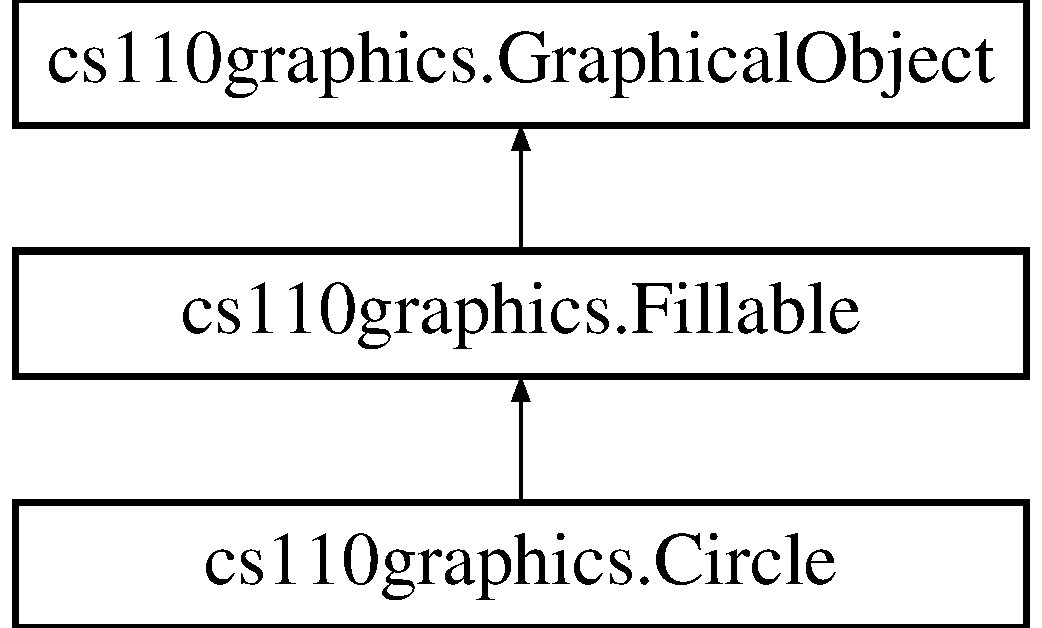
\includegraphics[height=3cm]{classcs110graphics_1_1Circle}
\end{center}
\end{figure}
\subsection*{Public Member Functions}
\begin{DoxyCompactItemize}
\item 
\hypertarget{classcs110graphics_1_1Circle_a7c92c173c0e9666d0682c48fbd170e9f}{
def {\bfseries \_\-\_\-init\_\-\_\-}}
\label{classcs110graphics_1_1Circle_a7c92c173c0e9666d0682c48fbd170e9f}

\item 
def \hyperlink{classcs110graphics_1_1Circle_a39b0cb138b31565d2a52180a2b03cc31}{set\_\-radius}
\begin{DoxyCompactList}\small\item\em Sets the radius of the \hyperlink{classcs110graphics_1_1Circle}{Circle}. \item\end{DoxyCompactList}\end{DoxyCompactItemize}


\subsection{Detailed Description}
A circle, which can be added to a \hyperlink{classcs110graphics_1_1Window}{Window} object. Required Parameters:
\begin{DoxyItemize}
\item window -\/ \hyperlink{classcs110graphics_1_1Window}{Window} -\/ the window which the object will be added to.
\end{DoxyItemize}

Optional Parameters:
\begin{DoxyItemize}
\item radius -\/ int -\/ sets the radius of the \hyperlink{classcs110graphics_1_1Circle}{Circle}. (default: 40)
\item center -\/ tuple -\/ sets the center of the \hyperlink{classcs110graphics_1_1Circle}{Circle}. (default: (200, 200)) 
\end{DoxyItemize}

\subsection{Member Function Documentation}
\hypertarget{classcs110graphics_1_1Circle_a39b0cb138b31565d2a52180a2b03cc31}{
\index{cs110graphics::Circle@{cs110graphics::Circle}!set\_\-radius@{set\_\-radius}}
\index{set\_\-radius@{set\_\-radius}!cs110graphics::Circle@{cs110graphics::Circle}}
\subsubsection[{set\_\-radius}]{\setlength{\rightskip}{0pt plus 5cm}def cs110graphics.Circle.set\_\-radius ( {\em self}, \/   {\em radius})}}
\label{classcs110graphics_1_1Circle_a39b0cb138b31565d2a52180a2b03cc31}


Sets the radius of the \hyperlink{classcs110graphics_1_1Circle}{Circle}. Required Parameters:
\begin{DoxyItemize}
\item radius -\/ int 
\end{DoxyItemize}

The documentation for this class was generated from the following file:\begin{DoxyCompactItemize}
\item 
cs110graphics.py\end{DoxyCompactItemize}

\hypertarget{classcs110graphics_1_1Event}{
\section{cs110graphics.Event Class Reference}
\label{classcs110graphics_1_1Event}\index{cs110graphics::Event@{cs110graphics::Event}}
}


An event which gets bound to an object.  
\subsection*{Public Member Functions}
\begin{DoxyCompactItemize}
\item 
\hypertarget{classcs110graphics_1_1Event_a79559b269fdb9c2252dfce99118455be}{
def {\bfseries \_\-\_\-init\_\-\_\-}}
\label{classcs110graphics_1_1Event_a79559b269fdb9c2252dfce99118455be}

\item 
def \hyperlink{classcs110graphics_1_1Event_abdb7a2999936cc7ab1119289f05f8243}{get\_\-button}
\begin{DoxyCompactList}\small\item\em Returns the mouse button that is attached to the event. \item\end{DoxyCompactList}\item 
def \hyperlink{classcs110graphics_1_1Event_a7bd201ecbf74db6d78dbf2fb4f622a7c}{get\_\-description}
\begin{DoxyCompactList}\small\item\em Returns the description of the event. \item\end{DoxyCompactList}\item 
def \hyperlink{classcs110graphics_1_1Event_a0d795ddaef92049cee1d7b09898cf225}{get\_\-key}
\begin{DoxyCompactList}\small\item\em Returns the keyboard key that is attached to the event. \item\end{DoxyCompactList}\item 
def \hyperlink{classcs110graphics_1_1Event_a2db4866adee7a6ddb8d32240801fb8ce}{get\_\-mouse\_\-location}
\begin{DoxyCompactList}\small\item\em Returns a tuple of the x and y coordinates of the mouse location in the canvas. \item\end{DoxyCompactList}\item 
def \hyperlink{classcs110graphics_1_1Event_a7c8fb2d5e9288db125801d5a6e66ecf1}{get\_\-root\_\-mouse\_\-location}
\begin{DoxyCompactList}\small\item\em Returns a tuple of the x and y coordinates of the mouse location in the window. \item\end{DoxyCompactList}\end{DoxyCompactItemize}


\subsection{Detailed Description}
An event which gets bound to an object. Used by \hyperlink{classcs110graphics_1_1EventHandler}{EventHandler} objects.

Required Parameters:
\begin{DoxyItemize}
\item event -\/ TkEvent -\/ The event which the user want applied an an object. 
\end{DoxyItemize}

\subsection{Member Function Documentation}
\hypertarget{classcs110graphics_1_1Event_abdb7a2999936cc7ab1119289f05f8243}{
\index{cs110graphics::Event@{cs110graphics::Event}!get\_\-button@{get\_\-button}}
\index{get\_\-button@{get\_\-button}!cs110graphics::Event@{cs110graphics::Event}}
\subsubsection[{get\_\-button}]{\setlength{\rightskip}{0pt plus 5cm}def cs110graphics.Event.get\_\-button ( {\em self})}}
\label{classcs110graphics_1_1Event_abdb7a2999936cc7ab1119289f05f8243}


Returns the mouse button that is attached to the event. Returns None if the button fails to exist (like if the \hyperlink{classcs110graphics_1_1Event}{Event} handles a key press). \hypertarget{classcs110graphics_1_1Event_a7bd201ecbf74db6d78dbf2fb4f622a7c}{
\index{cs110graphics::Event@{cs110graphics::Event}!get\_\-description@{get\_\-description}}
\index{get\_\-description@{get\_\-description}!cs110graphics::Event@{cs110graphics::Event}}
\subsubsection[{get\_\-description}]{\setlength{\rightskip}{0pt plus 5cm}def cs110graphics.Event.get\_\-description ( {\em self})}}
\label{classcs110graphics_1_1Event_a7bd201ecbf74db6d78dbf2fb4f622a7c}


Returns the description of the event. \hypertarget{classcs110graphics_1_1Event_a0d795ddaef92049cee1d7b09898cf225}{
\index{cs110graphics::Event@{cs110graphics::Event}!get\_\-key@{get\_\-key}}
\index{get\_\-key@{get\_\-key}!cs110graphics::Event@{cs110graphics::Event}}
\subsubsection[{get\_\-key}]{\setlength{\rightskip}{0pt plus 5cm}def cs110graphics.Event.get\_\-key ( {\em self})}}
\label{classcs110graphics_1_1Event_a0d795ddaef92049cee1d7b09898cf225}


Returns the keyboard key that is attached to the event. Returns None if the key fails to exist (like if the \hyperlink{classcs110graphics_1_1Event}{Event} handles a mouse press). \hypertarget{classcs110graphics_1_1Event_a2db4866adee7a6ddb8d32240801fb8ce}{
\index{cs110graphics::Event@{cs110graphics::Event}!get\_\-mouse\_\-location@{get\_\-mouse\_\-location}}
\index{get\_\-mouse\_\-location@{get\_\-mouse\_\-location}!cs110graphics::Event@{cs110graphics::Event}}
\subsubsection[{get\_\-mouse\_\-location}]{\setlength{\rightskip}{0pt plus 5cm}def cs110graphics.Event.get\_\-mouse\_\-location ( {\em self})}}
\label{classcs110graphics_1_1Event_a2db4866adee7a6ddb8d32240801fb8ce}


Returns a tuple of the x and y coordinates of the mouse location in the canvas. \hypertarget{classcs110graphics_1_1Event_a7c8fb2d5e9288db125801d5a6e66ecf1}{
\index{cs110graphics::Event@{cs110graphics::Event}!get\_\-root\_\-mouse\_\-location@{get\_\-root\_\-mouse\_\-location}}
\index{get\_\-root\_\-mouse\_\-location@{get\_\-root\_\-mouse\_\-location}!cs110graphics::Event@{cs110graphics::Event}}
\subsubsection[{get\_\-root\_\-mouse\_\-location}]{\setlength{\rightskip}{0pt plus 5cm}def cs110graphics.Event.get\_\-root\_\-mouse\_\-location ( {\em self})}}
\label{classcs110graphics_1_1Event_a7c8fb2d5e9288db125801d5a6e66ecf1}


Returns a tuple of the x and y coordinates of the mouse location in the window. 

The documentation for this class was generated from the following file:\begin{DoxyCompactItemize}
\item 
cs110graphics.py\end{DoxyCompactItemize}

\hypertarget{classcs110graphics_1_1EventHandler}{
\section{cs110graphics.EventHandler Class Reference}
\label{classcs110graphics_1_1EventHandler}\index{cs110graphics::EventHandler@{cs110graphics::EventHandler}}
}


Handles an event.  
\subsection*{Public Member Functions}
\begin{DoxyCompactItemize}
\item 
\hypertarget{classcs110graphics_1_1EventHandler_ad7fc16dbc70aae1a86f541b0e806da98}{
def {\bfseries \_\-\_\-init\_\-\_\-}}
\label{classcs110graphics_1_1EventHandler_ad7fc16dbc70aae1a86f541b0e806da98}

\item 
def \hyperlink{classcs110graphics_1_1EventHandler_af3fb3531d0b23f1430a830586cd07906}{handle\_\-key\_\-press}
\begin{DoxyCompactList}\small\item\em Handles a key press. \item\end{DoxyCompactList}\item 
def \hyperlink{classcs110graphics_1_1EventHandler_a6f5269e8062aaee8918560c637383c6e}{handke\_\-key\_\-release}
\begin{DoxyCompactList}\small\item\em Handles a key release. \item\end{DoxyCompactList}\item 
def \hyperlink{classcs110graphics_1_1EventHandler_a13af3268f8a1aa36b8483eb2deffef15}{handle\_\-mouse\_\-enter}
\begin{DoxyCompactList}\small\item\em Handles when a mouse enters an object. \item\end{DoxyCompactList}\item 
def \hyperlink{classcs110graphics_1_1EventHandler_a5deaf2b6b8055e97ac0ddf6603132c64}{handle\_\-mouse\_\-leave}
\begin{DoxyCompactList}\small\item\em Handles when a mouse leaves an object. \item\end{DoxyCompactList}\item 
def \hyperlink{classcs110graphics_1_1EventHandler_a521fdcd170d15c0b8baa124c78b6d1ef}{handle\_\-mouse\_\-move}
\begin{DoxyCompactList}\small\item\em Handles a mouse move. \item\end{DoxyCompactList}\item 
def \hyperlink{classcs110graphics_1_1EventHandler_a547873123ebcd3fcc63a2e03d2a2fee3}{handle\_\-mouse\_\-press}
\begin{DoxyCompactList}\small\item\em Handles a mouse press. \item\end{DoxyCompactList}\item 
def \hyperlink{classcs110graphics_1_1EventHandler_a320a7dbf68d37e0101b237bff1713088}{handle\_\-mouse\_\-release}
\begin{DoxyCompactList}\small\item\em Handles a mouse release. \item\end{DoxyCompactList}\end{DoxyCompactItemize}


\subsection{Detailed Description}
Handles an event. These are overloaded by the user, so by default they're empty except for the pass command. 

\subsection{Member Function Documentation}
\hypertarget{classcs110graphics_1_1EventHandler_a6f5269e8062aaee8918560c637383c6e}{
\index{cs110graphics::EventHandler@{cs110graphics::EventHandler}!handke\_\-key\_\-release@{handke\_\-key\_\-release}}
\index{handke\_\-key\_\-release@{handke\_\-key\_\-release}!cs110graphics::EventHandler@{cs110graphics::EventHandler}}
\subsubsection[{handke\_\-key\_\-release}]{\setlength{\rightskip}{0pt plus 5cm}def cs110graphics.EventHandler.handke\_\-key\_\-release ( {\em self}, \/   {\em event})}}
\label{classcs110graphics_1_1EventHandler_a6f5269e8062aaee8918560c637383c6e}


Handles a key release. Optional Parameters:
\begin{DoxyItemize}
\item event -\/ \hyperlink{classcs110graphics_1_1Event}{Event} -\/ when included, you can use any \hyperlink{classcs110graphics_1_1Event}{Event} method whenever this function is run. 
\end{DoxyItemize}\hypertarget{classcs110graphics_1_1EventHandler_af3fb3531d0b23f1430a830586cd07906}{
\index{cs110graphics::EventHandler@{cs110graphics::EventHandler}!handle\_\-key\_\-press@{handle\_\-key\_\-press}}
\index{handle\_\-key\_\-press@{handle\_\-key\_\-press}!cs110graphics::EventHandler@{cs110graphics::EventHandler}}
\subsubsection[{handle\_\-key\_\-press}]{\setlength{\rightskip}{0pt plus 5cm}def cs110graphics.EventHandler.handle\_\-key\_\-press ( {\em self}, \/   {\em event})}}
\label{classcs110graphics_1_1EventHandler_af3fb3531d0b23f1430a830586cd07906}


Handles a key press. Optional Parameters:
\begin{DoxyItemize}
\item event -\/ \hyperlink{classcs110graphics_1_1Event}{Event} -\/ when included, you can use any \hyperlink{classcs110graphics_1_1Event}{Event} method whenever this function is run. 
\end{DoxyItemize}\hypertarget{classcs110graphics_1_1EventHandler_a13af3268f8a1aa36b8483eb2deffef15}{
\index{cs110graphics::EventHandler@{cs110graphics::EventHandler}!handle\_\-mouse\_\-enter@{handle\_\-mouse\_\-enter}}
\index{handle\_\-mouse\_\-enter@{handle\_\-mouse\_\-enter}!cs110graphics::EventHandler@{cs110graphics::EventHandler}}
\subsubsection[{handle\_\-mouse\_\-enter}]{\setlength{\rightskip}{0pt plus 5cm}def cs110graphics.EventHandler.handle\_\-mouse\_\-enter ( {\em self}, \/   {\em event})}}
\label{classcs110graphics_1_1EventHandler_a13af3268f8a1aa36b8483eb2deffef15}


Handles when a mouse enters an object. Optional Parameters:
\begin{DoxyItemize}
\item event -\/ \hyperlink{classcs110graphics_1_1Event}{Event} -\/ when included, you can use any \hyperlink{classcs110graphics_1_1Event}{Event} method whenever this function is run. 
\end{DoxyItemize}\hypertarget{classcs110graphics_1_1EventHandler_a5deaf2b6b8055e97ac0ddf6603132c64}{
\index{cs110graphics::EventHandler@{cs110graphics::EventHandler}!handle\_\-mouse\_\-leave@{handle\_\-mouse\_\-leave}}
\index{handle\_\-mouse\_\-leave@{handle\_\-mouse\_\-leave}!cs110graphics::EventHandler@{cs110graphics::EventHandler}}
\subsubsection[{handle\_\-mouse\_\-leave}]{\setlength{\rightskip}{0pt plus 5cm}def cs110graphics.EventHandler.handle\_\-mouse\_\-leave ( {\em self}, \/   {\em event})}}
\label{classcs110graphics_1_1EventHandler_a5deaf2b6b8055e97ac0ddf6603132c64}


Handles when a mouse leaves an object. Optional Parameters:
\begin{DoxyItemize}
\item event -\/ \hyperlink{classcs110graphics_1_1Event}{Event} -\/ when included, you can use any \hyperlink{classcs110graphics_1_1Event}{Event} method whenever this function is run. 
\end{DoxyItemize}\hypertarget{classcs110graphics_1_1EventHandler_a521fdcd170d15c0b8baa124c78b6d1ef}{
\index{cs110graphics::EventHandler@{cs110graphics::EventHandler}!handle\_\-mouse\_\-move@{handle\_\-mouse\_\-move}}
\index{handle\_\-mouse\_\-move@{handle\_\-mouse\_\-move}!cs110graphics::EventHandler@{cs110graphics::EventHandler}}
\subsubsection[{handle\_\-mouse\_\-move}]{\setlength{\rightskip}{0pt plus 5cm}def cs110graphics.EventHandler.handle\_\-mouse\_\-move ( {\em self}, \/   {\em event})}}
\label{classcs110graphics_1_1EventHandler_a521fdcd170d15c0b8baa124c78b6d1ef}


Handles a mouse move. Optional Parameters:
\begin{DoxyItemize}
\item event -\/ \hyperlink{classcs110graphics_1_1Event}{Event} -\/ when included, you can use any \hyperlink{classcs110graphics_1_1Event}{Event} method whenever this function is run. 
\end{DoxyItemize}\hypertarget{classcs110graphics_1_1EventHandler_a547873123ebcd3fcc63a2e03d2a2fee3}{
\index{cs110graphics::EventHandler@{cs110graphics::EventHandler}!handle\_\-mouse\_\-press@{handle\_\-mouse\_\-press}}
\index{handle\_\-mouse\_\-press@{handle\_\-mouse\_\-press}!cs110graphics::EventHandler@{cs110graphics::EventHandler}}
\subsubsection[{handle\_\-mouse\_\-press}]{\setlength{\rightskip}{0pt plus 5cm}def cs110graphics.EventHandler.handle\_\-mouse\_\-press ( {\em self}, \/   {\em event})}}
\label{classcs110graphics_1_1EventHandler_a547873123ebcd3fcc63a2e03d2a2fee3}


Handles a mouse press. Optional Parameters:
\begin{DoxyItemize}
\item event -\/ \hyperlink{classcs110graphics_1_1Event}{Event} -\/ when included, you can use any \hyperlink{classcs110graphics_1_1Event}{Event} method whenever this function is run. 
\end{DoxyItemize}\hypertarget{classcs110graphics_1_1EventHandler_a320a7dbf68d37e0101b237bff1713088}{
\index{cs110graphics::EventHandler@{cs110graphics::EventHandler}!handle\_\-mouse\_\-release@{handle\_\-mouse\_\-release}}
\index{handle\_\-mouse\_\-release@{handle\_\-mouse\_\-release}!cs110graphics::EventHandler@{cs110graphics::EventHandler}}
\subsubsection[{handle\_\-mouse\_\-release}]{\setlength{\rightskip}{0pt plus 5cm}def cs110graphics.EventHandler.handle\_\-mouse\_\-release ( {\em self}, \/   {\em event})}}
\label{classcs110graphics_1_1EventHandler_a320a7dbf68d37e0101b237bff1713088}


Handles a mouse release. Optional Parameters:
\begin{DoxyItemize}
\item event -\/ \hyperlink{classcs110graphics_1_1Event}{Event} -\/ when included, you can use any \hyperlink{classcs110graphics_1_1Event}{Event} method whenever this function is run. 
\end{DoxyItemize}

The documentation for this class was generated from the following file:\begin{DoxyCompactItemize}
\item 
cs110graphics.py\end{DoxyCompactItemize}

\hypertarget{classcs110graphics_1_1Fillable}{
\section{cs110graphics.Fillable Class Reference}
\label{classcs110graphics_1_1Fillable}\index{cs110graphics::Fillable@{cs110graphics::Fillable}}
}


This window is a parent class of any object which can have its colors modified.  
Inheritance diagram for cs110graphics.Fillable::\begin{figure}[H]
\begin{center}
\leavevmode
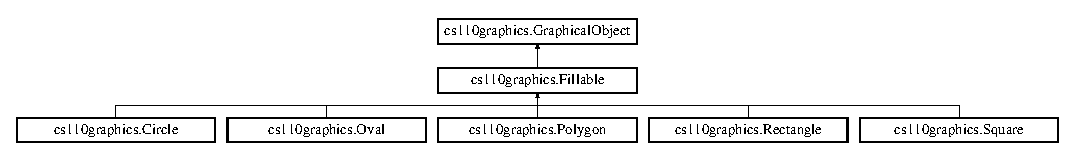
\includegraphics[height=1.68844cm]{classcs110graphics_1_1Fillable}
\end{center}
\end{figure}
\subsection*{Public Member Functions}
\begin{DoxyCompactItemize}
\item 
\hypertarget{classcs110graphics_1_1Fillable_a91e490828e9b9f0c3545af7fabf7a0b0}{
def {\bfseries \_\-\_\-init\_\-\_\-}}
\label{classcs110graphics_1_1Fillable_a91e490828e9b9f0c3545af7fabf7a0b0}

\item 
def \hyperlink{classcs110graphics_1_1Fillable_a6772d56158c9fe98a33f01d47cb8aa41}{get\_\-border\_\-color}
\begin{DoxyCompactList}\small\item\em Returns the border color of a \hyperlink{classcs110graphics_1_1Fillable}{Fillable}. \item\end{DoxyCompactList}\item 
def \hyperlink{classcs110graphics_1_1Fillable_a6ed7a4288e84a090ec185c8bdff21d0f}{get\_\-border\_\-width}
\begin{DoxyCompactList}\small\item\em Returns the border width of a \hyperlink{classcs110graphics_1_1Fillable}{Fillable}. \item\end{DoxyCompactList}\item 
def \hyperlink{classcs110graphics_1_1Fillable_a16c045bc9b63961b696914ee1a1d14d9}{get\_\-fill\_\-color}
\begin{DoxyCompactList}\small\item\em Returns the depth of a \hyperlink{classcs110graphics_1_1Fillable}{Fillable}. \item\end{DoxyCompactList}\item 
def \hyperlink{classcs110graphics_1_1Fillable_a514fa0d21297c1372681afae9219fd58}{get\_\-pivot}
\begin{DoxyCompactList}\small\item\em Returns the pivot point of a \hyperlink{classcs110graphics_1_1Fillable}{Fillable}. \item\end{DoxyCompactList}\item 
def \hyperlink{classcs110graphics_1_1Fillable_afa6710f6c314de39d19f06d9dd306d7d}{rotate}
\begin{DoxyCompactList}\small\item\em Rotates the object. \item\end{DoxyCompactList}\item 
def \hyperlink{classcs110graphics_1_1Fillable_a80d5b6b6d2ebae867dccecb803075749}{scale}
\begin{DoxyCompactList}\small\item\em Scales the \hyperlink{classcs110graphics_1_1Fillable}{Fillable} up or down depending on the factor. \item\end{DoxyCompactList}\item 
def \hyperlink{classcs110graphics_1_1Fillable_a2f830be5d970faac97759910d20d68a4}{set\_\-border\_\-color}
\begin{DoxyCompactList}\small\item\em Sets the border color of the \hyperlink{classcs110graphics_1_1Fillable}{Fillable}. \item\end{DoxyCompactList}\item 
def \hyperlink{classcs110graphics_1_1Fillable_a09f05462cb2ed38fdccb244340f05b2b}{set\_\-border\_\-width}
\begin{DoxyCompactList}\small\item\em Sets the border width of the \hyperlink{classcs110graphics_1_1Fillable}{Fillable}. \item\end{DoxyCompactList}\item 
def \hyperlink{classcs110graphics_1_1Fillable_a4f24c7186c8d057e42a0209eb1d56be7}{set\_\-fill\_\-color}
\begin{DoxyCompactList}\small\item\em Sets the fill color of the \hyperlink{classcs110graphics_1_1Fillable}{Fillable}. \item\end{DoxyCompactList}\item 
def \hyperlink{classcs110graphics_1_1Fillable_a2a6066d1a11c0854ff5ee85e7d9ceb54}{set\_\-pivot}
\begin{DoxyCompactList}\small\item\em Sets the pivot point of the \hyperlink{classcs110graphics_1_1Fillable}{Fillable}. \item\end{DoxyCompactList}\end{DoxyCompactItemize}


\subsection{Detailed Description}
This window is a parent class of any object which can have its colors modified. No constructor exists in this class, but its methods are used by other objects that extend/inherit this class. 

\subsection{Member Function Documentation}
\hypertarget{classcs110graphics_1_1Fillable_a6772d56158c9fe98a33f01d47cb8aa41}{
\index{cs110graphics::Fillable@{cs110graphics::Fillable}!get\_\-border\_\-color@{get\_\-border\_\-color}}
\index{get\_\-border\_\-color@{get\_\-border\_\-color}!cs110graphics::Fillable@{cs110graphics::Fillable}}
\subsubsection[{get\_\-border\_\-color}]{\setlength{\rightskip}{0pt plus 5cm}def cs110graphics.Fillable.get\_\-border\_\-color ( {\em self})}}
\label{classcs110graphics_1_1Fillable_a6772d56158c9fe98a33f01d47cb8aa41}


Returns the border color of a \hyperlink{classcs110graphics_1_1Fillable}{Fillable}. \hypertarget{classcs110graphics_1_1Fillable_a6ed7a4288e84a090ec185c8bdff21d0f}{
\index{cs110graphics::Fillable@{cs110graphics::Fillable}!get\_\-border\_\-width@{get\_\-border\_\-width}}
\index{get\_\-border\_\-width@{get\_\-border\_\-width}!cs110graphics::Fillable@{cs110graphics::Fillable}}
\subsubsection[{get\_\-border\_\-width}]{\setlength{\rightskip}{0pt plus 5cm}def cs110graphics.Fillable.get\_\-border\_\-width ( {\em self})}}
\label{classcs110graphics_1_1Fillable_a6ed7a4288e84a090ec185c8bdff21d0f}


Returns the border width of a \hyperlink{classcs110graphics_1_1Fillable}{Fillable}. \hypertarget{classcs110graphics_1_1Fillable_a16c045bc9b63961b696914ee1a1d14d9}{
\index{cs110graphics::Fillable@{cs110graphics::Fillable}!get\_\-fill\_\-color@{get\_\-fill\_\-color}}
\index{get\_\-fill\_\-color@{get\_\-fill\_\-color}!cs110graphics::Fillable@{cs110graphics::Fillable}}
\subsubsection[{get\_\-fill\_\-color}]{\setlength{\rightskip}{0pt plus 5cm}def cs110graphics.Fillable.get\_\-fill\_\-color ( {\em self})}}
\label{classcs110graphics_1_1Fillable_a16c045bc9b63961b696914ee1a1d14d9}


Returns the depth of a \hyperlink{classcs110graphics_1_1Fillable}{Fillable}. \hypertarget{classcs110graphics_1_1Fillable_a514fa0d21297c1372681afae9219fd58}{
\index{cs110graphics::Fillable@{cs110graphics::Fillable}!get\_\-pivot@{get\_\-pivot}}
\index{get\_\-pivot@{get\_\-pivot}!cs110graphics::Fillable@{cs110graphics::Fillable}}
\subsubsection[{get\_\-pivot}]{\setlength{\rightskip}{0pt plus 5cm}def cs110graphics.Fillable.get\_\-pivot ( {\em self})}}
\label{classcs110graphics_1_1Fillable_a514fa0d21297c1372681afae9219fd58}


Returns the pivot point of a \hyperlink{classcs110graphics_1_1Fillable}{Fillable}. \hypertarget{classcs110graphics_1_1Fillable_afa6710f6c314de39d19f06d9dd306d7d}{
\index{cs110graphics::Fillable@{cs110graphics::Fillable}!rotate@{rotate}}
\index{rotate@{rotate}!cs110graphics::Fillable@{cs110graphics::Fillable}}
\subsubsection[{rotate}]{\setlength{\rightskip}{0pt plus 5cm}def cs110graphics.Fillable.rotate ( {\em self}, \/   {\em degrees})}}
\label{classcs110graphics_1_1Fillable_afa6710f6c314de39d19f06d9dd306d7d}


Rotates the object. Required Parameters:
\begin{DoxyItemize}
\item degrees -\/ int 
\end{DoxyItemize}\hypertarget{classcs110graphics_1_1Fillable_a80d5b6b6d2ebae867dccecb803075749}{
\index{cs110graphics::Fillable@{cs110graphics::Fillable}!scale@{scale}}
\index{scale@{scale}!cs110graphics::Fillable@{cs110graphics::Fillable}}
\subsubsection[{scale}]{\setlength{\rightskip}{0pt plus 5cm}def cs110graphics.Fillable.scale ( {\em self}, \/   {\em factor})}}
\label{classcs110graphics_1_1Fillable_a80d5b6b6d2ebae867dccecb803075749}


Scales the \hyperlink{classcs110graphics_1_1Fillable}{Fillable} up or down depending on the factor. Required Parameters:
\begin{DoxyItemize}
\item factor -\/ float 
\end{DoxyItemize}\hypertarget{classcs110graphics_1_1Fillable_a2f830be5d970faac97759910d20d68a4}{
\index{cs110graphics::Fillable@{cs110graphics::Fillable}!set\_\-border\_\-color@{set\_\-border\_\-color}}
\index{set\_\-border\_\-color@{set\_\-border\_\-color}!cs110graphics::Fillable@{cs110graphics::Fillable}}
\subsubsection[{set\_\-border\_\-color}]{\setlength{\rightskip}{0pt plus 5cm}def cs110graphics.Fillable.set\_\-border\_\-color ( {\em self}, \/   {\em color})}}
\label{classcs110graphics_1_1Fillable_a2f830be5d970faac97759910d20d68a4}


Sets the border color of the \hyperlink{classcs110graphics_1_1Fillable}{Fillable}. Required Parameters:
\begin{DoxyItemize}
\item color -\/ string 
\end{DoxyItemize}\hypertarget{classcs110graphics_1_1Fillable_a09f05462cb2ed38fdccb244340f05b2b}{
\index{cs110graphics::Fillable@{cs110graphics::Fillable}!set\_\-border\_\-width@{set\_\-border\_\-width}}
\index{set\_\-border\_\-width@{set\_\-border\_\-width}!cs110graphics::Fillable@{cs110graphics::Fillable}}
\subsubsection[{set\_\-border\_\-width}]{\setlength{\rightskip}{0pt plus 5cm}def cs110graphics.Fillable.set\_\-border\_\-width ( {\em self}, \/   {\em width})}}
\label{classcs110graphics_1_1Fillable_a09f05462cb2ed38fdccb244340f05b2b}


Sets the border width of the \hyperlink{classcs110graphics_1_1Fillable}{Fillable}. Required Parameters:
\begin{DoxyItemize}
\item width -\/ int 
\end{DoxyItemize}\hypertarget{classcs110graphics_1_1Fillable_a4f24c7186c8d057e42a0209eb1d56be7}{
\index{cs110graphics::Fillable@{cs110graphics::Fillable}!set\_\-fill\_\-color@{set\_\-fill\_\-color}}
\index{set\_\-fill\_\-color@{set\_\-fill\_\-color}!cs110graphics::Fillable@{cs110graphics::Fillable}}
\subsubsection[{set\_\-fill\_\-color}]{\setlength{\rightskip}{0pt plus 5cm}def cs110graphics.Fillable.set\_\-fill\_\-color ( {\em self}, \/   {\em color})}}
\label{classcs110graphics_1_1Fillable_a4f24c7186c8d057e42a0209eb1d56be7}


Sets the fill color of the \hyperlink{classcs110graphics_1_1Fillable}{Fillable}. Required Parameters:
\begin{DoxyItemize}
\item color -\/ string 
\end{DoxyItemize}\hypertarget{classcs110graphics_1_1Fillable_a2a6066d1a11c0854ff5ee85e7d9ceb54}{
\index{cs110graphics::Fillable@{cs110graphics::Fillable}!set\_\-pivot@{set\_\-pivot}}
\index{set\_\-pivot@{set\_\-pivot}!cs110graphics::Fillable@{cs110graphics::Fillable}}
\subsubsection[{set\_\-pivot}]{\setlength{\rightskip}{0pt plus 5cm}def cs110graphics.Fillable.set\_\-pivot ( {\em self}, \/   {\em pivot})}}
\label{classcs110graphics_1_1Fillable_a2a6066d1a11c0854ff5ee85e7d9ceb54}


Sets the pivot point of the \hyperlink{classcs110graphics_1_1Fillable}{Fillable}. Required Parameters:
\begin{DoxyItemize}
\item pivot -\/ tuple of (int $\ast$ int) 
\end{DoxyItemize}

The documentation for this class was generated from the following file:\begin{DoxyCompactItemize}
\item 
cs110graphics.py\end{DoxyCompactItemize}

\hypertarget{classcs110graphics_1_1GraphicalObject}{
\section{cs110graphics.GraphicalObject Class Reference}
\label{classcs110graphics_1_1GraphicalObject}\index{cs110graphics::GraphicalObject@{cs110graphics::GraphicalObject}}
}


This window is a parent class of any object which can be put into \hyperlink{classcs110graphics_1_1Window}{Window}.  
Inheritance diagram for cs110graphics.GraphicalObject::\begin{figure}[H]
\begin{center}
\leavevmode
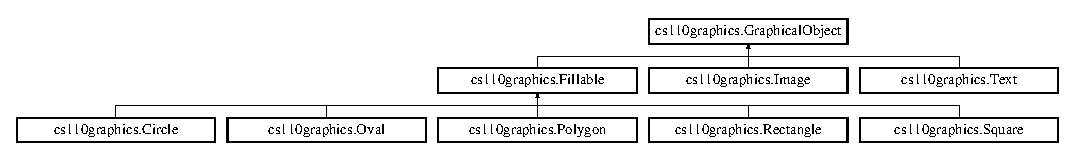
\includegraphics[height=1.68844cm]{classcs110graphics_1_1GraphicalObject}
\end{center}
\end{figure}
\subsection*{Public Member Functions}
\begin{DoxyCompactItemize}
\item 
\hypertarget{classcs110graphics_1_1GraphicalObject_a1c84a127a5d1cae5802e326b9b024140}{
def {\bfseries \_\-\_\-init\_\-\_\-}}
\label{classcs110graphics_1_1GraphicalObject_a1c84a127a5d1cae5802e326b9b024140}

\item 
def \hyperlink{classcs110graphics_1_1GraphicalObject_adb1af0d5a6baae3f9a08d21a3227c49f}{add\_\-handler}
\begin{DoxyCompactList}\small\item\em Adds a handler to the graphical object. \item\end{DoxyCompactList}\item 
def \hyperlink{classcs110graphics_1_1GraphicalObject_a062789c4cc9de38af32dcc4ff2058607}{get\_\-center}
\begin{DoxyCompactList}\small\item\em Returns the center of the graphical object. \item\end{DoxyCompactList}\item 
def \hyperlink{classcs110graphics_1_1GraphicalObject_a6d9f5718cd0cf249e0d2842971bae17f}{get\_\-depth}
\begin{DoxyCompactList}\small\item\em Returns the depth of the graphical object. \item\end{DoxyCompactList}\item 
def \hyperlink{classcs110graphics_1_1GraphicalObject_aa64d270fb83efa4a54e1a7953512f9cd}{move}
\begin{DoxyCompactList}\small\item\em Moves a graphical object dx pixels horizontally and dy pixels vertically. \item\end{DoxyCompactList}\item 
def \hyperlink{classcs110graphics_1_1GraphicalObject_abe2d480265df7ac9447205c52c6946df}{move\_\-to}
\begin{DoxyCompactList}\small\item\em Moves a graphical object to a point. \item\end{DoxyCompactList}\item 
def \hyperlink{classcs110graphics_1_1GraphicalObject_a20d76d4ee4419c3065d61deb6cbc6700}{set\_\-depth}
\begin{DoxyCompactList}\small\item\em Sets the depth of the \hyperlink{classcs110graphics_1_1GraphicalObject}{GraphicalObject}. \item\end{DoxyCompactList}\end{DoxyCompactItemize}


\subsection{Detailed Description}
This window is a parent class of any object which can be put into \hyperlink{classcs110graphics_1_1Window}{Window}. No constructor exists in this class, but its methods are used by other objects that extend/inherit this class. 

\subsection{Member Function Documentation}
\hypertarget{classcs110graphics_1_1GraphicalObject_adb1af0d5a6baae3f9a08d21a3227c49f}{
\index{cs110graphics::GraphicalObject@{cs110graphics::GraphicalObject}!add\_\-handler@{add\_\-handler}}
\index{add\_\-handler@{add\_\-handler}!cs110graphics::GraphicalObject@{cs110graphics::GraphicalObject}}
\subsubsection[{add\_\-handler}]{\setlength{\rightskip}{0pt plus 5cm}def cs110graphics.GraphicalObject.add\_\-handler ( {\em self}, \/   {\em handler\_\-object})}}
\label{classcs110graphics_1_1GraphicalObject_adb1af0d5a6baae3f9a08d21a3227c49f}


Adds a handler to the graphical object. Required Parameters:
\begin{DoxyItemize}
\item handler\_\-object -\/ an object with a \hyperlink{classcs110graphics_1_1GraphicalObject}{GraphicalObject} representation within it (such as an object which has a \hyperlink{classcs110graphics_1_1Circle}{Circle} object in it) 
\end{DoxyItemize}\hypertarget{classcs110graphics_1_1GraphicalObject_a062789c4cc9de38af32dcc4ff2058607}{
\index{cs110graphics::GraphicalObject@{cs110graphics::GraphicalObject}!get\_\-center@{get\_\-center}}
\index{get\_\-center@{get\_\-center}!cs110graphics::GraphicalObject@{cs110graphics::GraphicalObject}}
\subsubsection[{get\_\-center}]{\setlength{\rightskip}{0pt plus 5cm}def cs110graphics.GraphicalObject.get\_\-center ( {\em self})}}
\label{classcs110graphics_1_1GraphicalObject_a062789c4cc9de38af32dcc4ff2058607}


Returns the center of the graphical object. \hypertarget{classcs110graphics_1_1GraphicalObject_a6d9f5718cd0cf249e0d2842971bae17f}{
\index{cs110graphics::GraphicalObject@{cs110graphics::GraphicalObject}!get\_\-depth@{get\_\-depth}}
\index{get\_\-depth@{get\_\-depth}!cs110graphics::GraphicalObject@{cs110graphics::GraphicalObject}}
\subsubsection[{get\_\-depth}]{\setlength{\rightskip}{0pt plus 5cm}def cs110graphics.GraphicalObject.get\_\-depth ( {\em self})}}
\label{classcs110graphics_1_1GraphicalObject_a6d9f5718cd0cf249e0d2842971bae17f}


Returns the depth of the graphical object. \hypertarget{classcs110graphics_1_1GraphicalObject_aa64d270fb83efa4a54e1a7953512f9cd}{
\index{cs110graphics::GraphicalObject@{cs110graphics::GraphicalObject}!move@{move}}
\index{move@{move}!cs110graphics::GraphicalObject@{cs110graphics::GraphicalObject}}
\subsubsection[{move}]{\setlength{\rightskip}{0pt plus 5cm}def cs110graphics.GraphicalObject.move ( {\em self}, \/   {\em dx}, \/   {\em dy})}}
\label{classcs110graphics_1_1GraphicalObject_aa64d270fb83efa4a54e1a7953512f9cd}


Moves a graphical object dx pixels horizontally and dy pixels vertically. Required Parameters:
\begin{DoxyItemize}
\item dx -\/ int
\item dy -\/ int 
\end{DoxyItemize}

Reimplemented in \hyperlink{classcs110graphics_1_1Image_a540d48247976343a91c610009a9af8cd}{cs110graphics.Image}, and \hyperlink{classcs110graphics_1_1Text_a6bd6f174fc82f2225a4d162ca6b90ec2}{cs110graphics.Text}.\hypertarget{classcs110graphics_1_1GraphicalObject_abe2d480265df7ac9447205c52c6946df}{
\index{cs110graphics::GraphicalObject@{cs110graphics::GraphicalObject}!move\_\-to@{move\_\-to}}
\index{move\_\-to@{move\_\-to}!cs110graphics::GraphicalObject@{cs110graphics::GraphicalObject}}
\subsubsection[{move\_\-to}]{\setlength{\rightskip}{0pt plus 5cm}def cs110graphics.GraphicalObject.move\_\-to ( {\em self}, \/   {\em point})}}
\label{classcs110graphics_1_1GraphicalObject_abe2d480265df7ac9447205c52c6946df}


Moves a graphical object to a point. Required Parameters:
\begin{DoxyItemize}
\item point -\/ tuple of (int $\ast$ int) 
\end{DoxyItemize}

Reimplemented in \hyperlink{classcs110graphics_1_1Image_a4b2e775fbb0cb523f6bc09028dc05c65}{cs110graphics.Image}, and \hyperlink{classcs110graphics_1_1Text_a615a76c8d2edd6c6af5d39d4e2577a27}{cs110graphics.Text}.\hypertarget{classcs110graphics_1_1GraphicalObject_a20d76d4ee4419c3065d61deb6cbc6700}{
\index{cs110graphics::GraphicalObject@{cs110graphics::GraphicalObject}!set\_\-depth@{set\_\-depth}}
\index{set\_\-depth@{set\_\-depth}!cs110graphics::GraphicalObject@{cs110graphics::GraphicalObject}}
\subsubsection[{set\_\-depth}]{\setlength{\rightskip}{0pt plus 5cm}def cs110graphics.GraphicalObject.set\_\-depth ( {\em self}, \/   {\em depth})}}
\label{classcs110graphics_1_1GraphicalObject_a20d76d4ee4419c3065d61deb6cbc6700}


Sets the depth of the \hyperlink{classcs110graphics_1_1GraphicalObject}{GraphicalObject}. Required Parameters:
\begin{DoxyItemize}
\item depth -\/ int 
\end{DoxyItemize}

The documentation for this class was generated from the following file:\begin{DoxyCompactItemize}
\item 
cs110graphics.py\end{DoxyCompactItemize}

\hypertarget{classcs110graphics_1_1Image}{
\section{cs110graphics.Image Class Reference}
\label{classcs110graphics_1_1Image}\index{cs110graphics::Image@{cs110graphics::Image}}
}


An image, which can be added to a \hyperlink{classcs110graphics_1_1Window}{Window} object.  
Inheritance diagram for cs110graphics.Image::\begin{figure}[H]
\begin{center}
\leavevmode
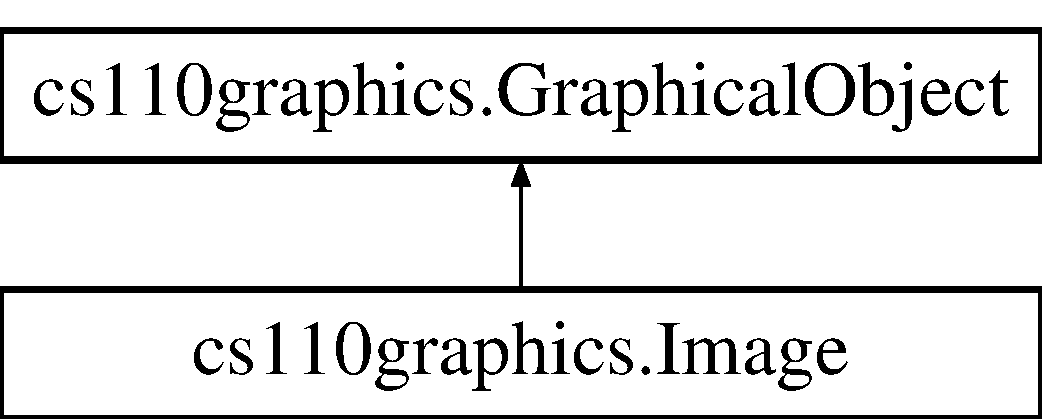
\includegraphics[height=2cm]{classcs110graphics_1_1Image}
\end{center}
\end{figure}
\subsection*{Public Member Functions}
\begin{DoxyCompactItemize}
\item 
\hypertarget{classcs110graphics_1_1Image_a3b7c128fa18d85ff4a7586fac04a1bc2}{
def {\bfseries \_\-\_\-init\_\-\_\-}}
\label{classcs110graphics_1_1Image_a3b7c128fa18d85ff4a7586fac04a1bc2}

\item 
def \hyperlink{classcs110graphics_1_1Image_a540d48247976343a91c610009a9af8cd}{move}
\begin{DoxyCompactList}\small\item\em Moves a graphical object dx pixels horizontally and dy pixels vertically. \item\end{DoxyCompactList}\item 
def \hyperlink{classcs110graphics_1_1Image_a4b2e775fbb0cb523f6bc09028dc05c65}{move\_\-to}
\begin{DoxyCompactList}\small\item\em Moves a graphical object to a point. \item\end{DoxyCompactList}\item 
def \hyperlink{classcs110graphics_1_1Image_a0754151035bb2892f0cd3895b64488fa}{resize}
\begin{DoxyCompactList}\small\item\em Resizes the \hyperlink{classcs110graphics_1_1Image}{Image}. \item\end{DoxyCompactList}\item 
def \hyperlink{classcs110graphics_1_1Image_ac58717d68279e536cee608e2bdfc6aa8}{rotate}
\begin{DoxyCompactList}\small\item\em Rotates an object by degrees. \item\end{DoxyCompactList}\item 
def \hyperlink{classcs110graphics_1_1Image_a7a59fde33fe83916a4155fafb5cfb01e}{scale}
\begin{DoxyCompactList}\small\item\em Scales the image according to the factor. \item\end{DoxyCompactList}\item 
def \hyperlink{classcs110graphics_1_1Image_a4ff2da7a167a433f2c38f1e2e2fe7263}{size}
\begin{DoxyCompactList}\small\item\em Returns a tuple of the width and height of the image. \item\end{DoxyCompactList}\end{DoxyCompactItemize}


\subsection{Detailed Description}
An image, which can be added to a \hyperlink{classcs110graphics_1_1Window}{Window} object. Required Parameters:
\begin{DoxyItemize}
\item window -\/ \hyperlink{classcs110graphics_1_1Window}{Window} -\/ the window which the object will be added to.
\item image\_\-loc -\/ str -\/ The name of an image within the current working directory. (If the current working directory is /foo/bar, then the image the user wants to use has to be in that directory. There is no support for using internet links at this time.)
\end{DoxyItemize}

Optional Parameters:
\begin{DoxyItemize}
\item center -\/ tuple of int $\ast$ int -\/ sets the center of the \hyperlink{classcs110graphics_1_1Image}{Image}. (default: (200, 200))
\item width -\/ int -\/ sets the width of the image. (default: 25)
\item height -\/ int -\/ sets the height of the image. (default: 25) 
\end{DoxyItemize}

\subsection{Member Function Documentation}
\hypertarget{classcs110graphics_1_1Image_a540d48247976343a91c610009a9af8cd}{
\index{cs110graphics::Image@{cs110graphics::Image}!move@{move}}
\index{move@{move}!cs110graphics::Image@{cs110graphics::Image}}
\subsubsection[{move}]{\setlength{\rightskip}{0pt plus 5cm}def cs110graphics.Image.move ( {\em self}, \/   {\em dx}, \/   {\em dy})}}
\label{classcs110graphics_1_1Image_a540d48247976343a91c610009a9af8cd}


Moves a graphical object dx pixels horizontally and dy pixels vertically. Required Parameters:
\begin{DoxyItemize}
\item dx -\/ int
\item dy -\/ int 
\end{DoxyItemize}

Reimplemented from \hyperlink{classcs110graphics_1_1GraphicalObject_aa64d270fb83efa4a54e1a7953512f9cd}{cs110graphics.GraphicalObject}.\hypertarget{classcs110graphics_1_1Image_a4b2e775fbb0cb523f6bc09028dc05c65}{
\index{cs110graphics::Image@{cs110graphics::Image}!move\_\-to@{move\_\-to}}
\index{move\_\-to@{move\_\-to}!cs110graphics::Image@{cs110graphics::Image}}
\subsubsection[{move\_\-to}]{\setlength{\rightskip}{0pt plus 5cm}def cs110graphics.Image.move\_\-to ( {\em self}, \/   {\em point})}}
\label{classcs110graphics_1_1Image_a4b2e775fbb0cb523f6bc09028dc05c65}


Moves a graphical object to a point. Required Parameters:
\begin{DoxyItemize}
\item point -\/ tuple of (int $\ast$ int) 
\end{DoxyItemize}

Reimplemented from \hyperlink{classcs110graphics_1_1GraphicalObject_abe2d480265df7ac9447205c52c6946df}{cs110graphics.GraphicalObject}.\hypertarget{classcs110graphics_1_1Image_a0754151035bb2892f0cd3895b64488fa}{
\index{cs110graphics::Image@{cs110graphics::Image}!resize@{resize}}
\index{resize@{resize}!cs110graphics::Image@{cs110graphics::Image}}
\subsubsection[{resize}]{\setlength{\rightskip}{0pt plus 5cm}def cs110graphics.Image.resize ( {\em self}, \/   {\em width}, \/   {\em height})}}
\label{classcs110graphics_1_1Image_a0754151035bb2892f0cd3895b64488fa}


Resizes the \hyperlink{classcs110graphics_1_1Image}{Image}. Required Parameters:
\begin{DoxyItemize}
\item width -\/ int
\item height -\/ int 
\end{DoxyItemize}\hypertarget{classcs110graphics_1_1Image_ac58717d68279e536cee608e2bdfc6aa8}{
\index{cs110graphics::Image@{cs110graphics::Image}!rotate@{rotate}}
\index{rotate@{rotate}!cs110graphics::Image@{cs110graphics::Image}}
\subsubsection[{rotate}]{\setlength{\rightskip}{0pt plus 5cm}def cs110graphics.Image.rotate ( {\em self}, \/   {\em degrees})}}
\label{classcs110graphics_1_1Image_ac58717d68279e536cee608e2bdfc6aa8}


Rotates an object by degrees. Required Parameters:
\begin{DoxyItemize}
\item degrees -\/ int 
\end{DoxyItemize}\hypertarget{classcs110graphics_1_1Image_a7a59fde33fe83916a4155fafb5cfb01e}{
\index{cs110graphics::Image@{cs110graphics::Image}!scale@{scale}}
\index{scale@{scale}!cs110graphics::Image@{cs110graphics::Image}}
\subsubsection[{scale}]{\setlength{\rightskip}{0pt plus 5cm}def cs110graphics.Image.scale ( {\em self}, \/   {\em factor})}}
\label{classcs110graphics_1_1Image_a7a59fde33fe83916a4155fafb5cfb01e}


Scales the image according to the factor. Required Parameters:
\begin{DoxyItemize}
\item factor -\/ float 
\end{DoxyItemize}\hypertarget{classcs110graphics_1_1Image_a4ff2da7a167a433f2c38f1e2e2fe7263}{
\index{cs110graphics::Image@{cs110graphics::Image}!size@{size}}
\index{size@{size}!cs110graphics::Image@{cs110graphics::Image}}
\subsubsection[{size}]{\setlength{\rightskip}{0pt plus 5cm}def cs110graphics.Image.size ( {\em self})}}
\label{classcs110graphics_1_1Image_a4ff2da7a167a433f2c38f1e2e2fe7263}


Returns a tuple of the width and height of the image. 

The documentation for this class was generated from the following file:\begin{DoxyCompactItemize}
\item 
cs110graphics.py\end{DoxyCompactItemize}

\hypertarget{classcs110graphics_1_1Oval}{
\section{cs110graphics.Oval Class Reference}
\label{classcs110graphics_1_1Oval}\index{cs110graphics::Oval@{cs110graphics::Oval}}
}


An oval, which can be added to a \hyperlink{classcs110graphics_1_1Window}{Window} object.  
Inheritance diagram for cs110graphics.Oval::\begin{figure}[H]
\begin{center}
\leavevmode
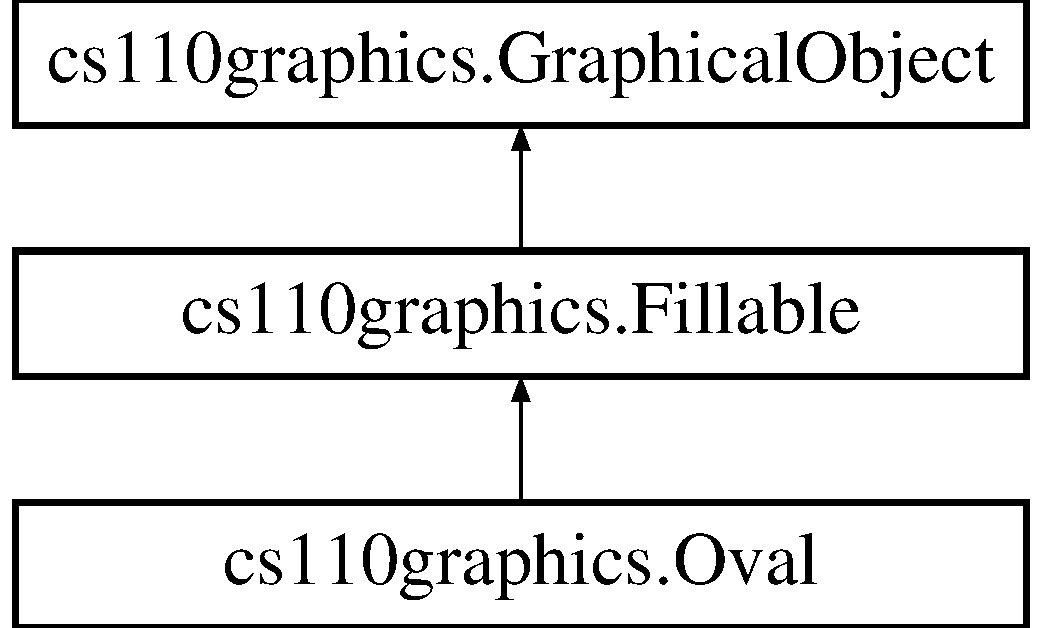
\includegraphics[height=3cm]{classcs110graphics_1_1Oval}
\end{center}
\end{figure}
\subsection*{Public Member Functions}
\begin{DoxyCompactItemize}
\item 
\hypertarget{classcs110graphics_1_1Oval_a7f71ea6ad224b510456c9de76e72ff11}{
def {\bfseries \_\-\_\-init\_\-\_\-}}
\label{classcs110graphics_1_1Oval_a7f71ea6ad224b510456c9de76e72ff11}

\item 
def \hyperlink{classcs110graphics_1_1Oval_a5d699cffc26c514e0eb9bdfde9a2951b}{set\_\-radii}
\begin{DoxyCompactList}\small\item\em Sets the horizontal and vertical radii of the \hyperlink{classcs110graphics_1_1Oval}{Oval}. \item\end{DoxyCompactList}\end{DoxyCompactItemize}


\subsection{Detailed Description}
An oval, which can be added to a \hyperlink{classcs110graphics_1_1Window}{Window} object. Required Parameters:
\begin{DoxyItemize}
\item window -\/ \hyperlink{classcs110graphics_1_1Window}{Window} -\/ the window which the object will be added to.
\end{DoxyItemize}

Optional Parameters:
\begin{DoxyItemize}
\item radiusX -\/ int -\/ sets the radius of the \hyperlink{classcs110graphics_1_1Oval}{Oval}. (default: 40)
\item radiusY -\/ int -\/ sets the radius of the \hyperlink{classcs110graphics_1_1Oval}{Oval}. (default: 60)
\item center -\/ tuple -\/ sets the center of the \hyperlink{classcs110graphics_1_1Oval}{Oval}. (default: (200, 200)) 
\end{DoxyItemize}

\subsection{Member Function Documentation}
\hypertarget{classcs110graphics_1_1Oval_a5d699cffc26c514e0eb9bdfde9a2951b}{
\index{cs110graphics::Oval@{cs110graphics::Oval}!set\_\-radii@{set\_\-radii}}
\index{set\_\-radii@{set\_\-radii}!cs110graphics::Oval@{cs110graphics::Oval}}
\subsubsection[{set\_\-radii}]{\setlength{\rightskip}{0pt plus 5cm}def cs110graphics.Oval.set\_\-radii ( {\em self}, \/   {\em radiusX}, \/   {\em radiusY})}}
\label{classcs110graphics_1_1Oval_a5d699cffc26c514e0eb9bdfde9a2951b}


Sets the horizontal and vertical radii of the \hyperlink{classcs110graphics_1_1Oval}{Oval}. Required Parameters:
\begin{DoxyItemize}
\item radiusX -\/ int
\item radiusY -\/ int 
\end{DoxyItemize}

The documentation for this class was generated from the following file:\begin{DoxyCompactItemize}
\item 
cs110graphics.py\end{DoxyCompactItemize}

\hypertarget{classcs110graphics_1_1Polygon}{
\section{cs110graphics.Polygon Class Reference}
\label{classcs110graphics_1_1Polygon}\index{cs110graphics::Polygon@{cs110graphics::Polygon}}
}


A \hyperlink{classcs110graphics_1_1Polygon}{Polygon}, which can be added to a \hyperlink{classcs110graphics_1_1Window}{Window} object.  
Inheritance diagram for cs110graphics.Polygon::\begin{figure}[H]
\begin{center}
\leavevmode
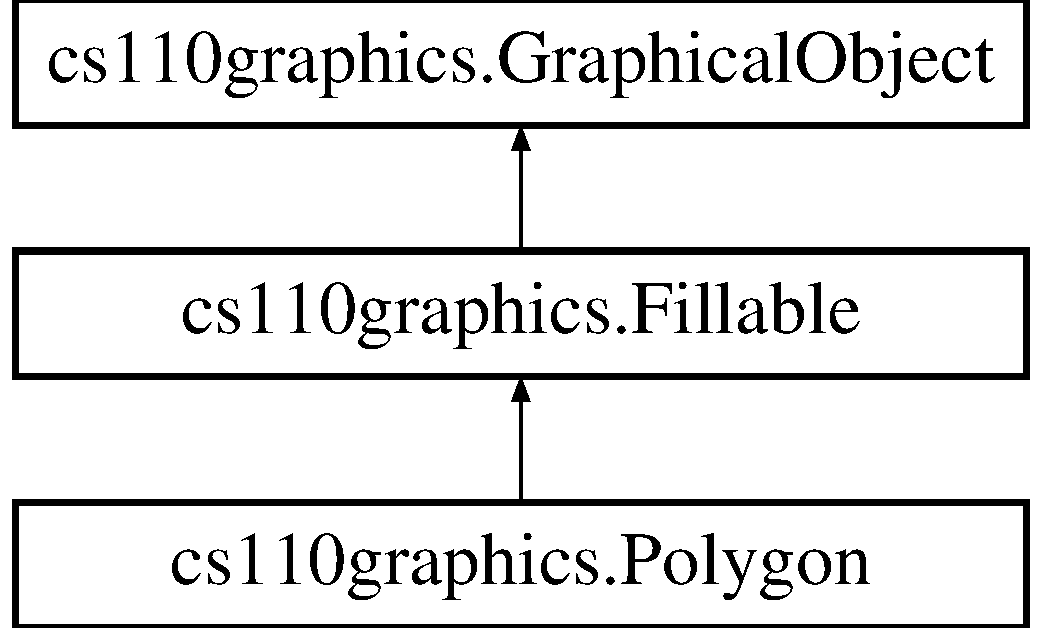
\includegraphics[height=3cm]{classcs110graphics_1_1Polygon}
\end{center}
\end{figure}
\subsection*{Public Member Functions}
\begin{DoxyCompactItemize}
\item 
\hypertarget{classcs110graphics_1_1Polygon_ab471e73072b87896eec42f385102c800}{
def {\bfseries \_\-\_\-init\_\-\_\-}}
\label{classcs110graphics_1_1Polygon_ab471e73072b87896eec42f385102c800}

\end{DoxyCompactItemize}


\subsection{Detailed Description}
A \hyperlink{classcs110graphics_1_1Polygon}{Polygon}, which can be added to a \hyperlink{classcs110graphics_1_1Window}{Window} object. Required Parameters:
\begin{DoxyItemize}
\item window -\/ \hyperlink{classcs110graphics_1_1Window}{Window} -\/ the window which the object will be added to.
\item points -\/ list of tuples of int $\ast$ int -\/ each tuple corresponds to an xy point. 
\end{DoxyItemize}

The documentation for this class was generated from the following file:\begin{DoxyCompactItemize}
\item 
cs110graphics.py\end{DoxyCompactItemize}

\hypertarget{classcs110graphics_1_1Rectangle}{
\section{cs110graphics.Rectangle Class Reference}
\label{classcs110graphics_1_1Rectangle}\index{cs110graphics::Rectangle@{cs110graphics::Rectangle}}
}


A rectangle, which can be added to a \hyperlink{classcs110graphics_1_1Window}{Window} object.  
Inheritance diagram for cs110graphics.Rectangle::\begin{figure}[H]
\begin{center}
\leavevmode
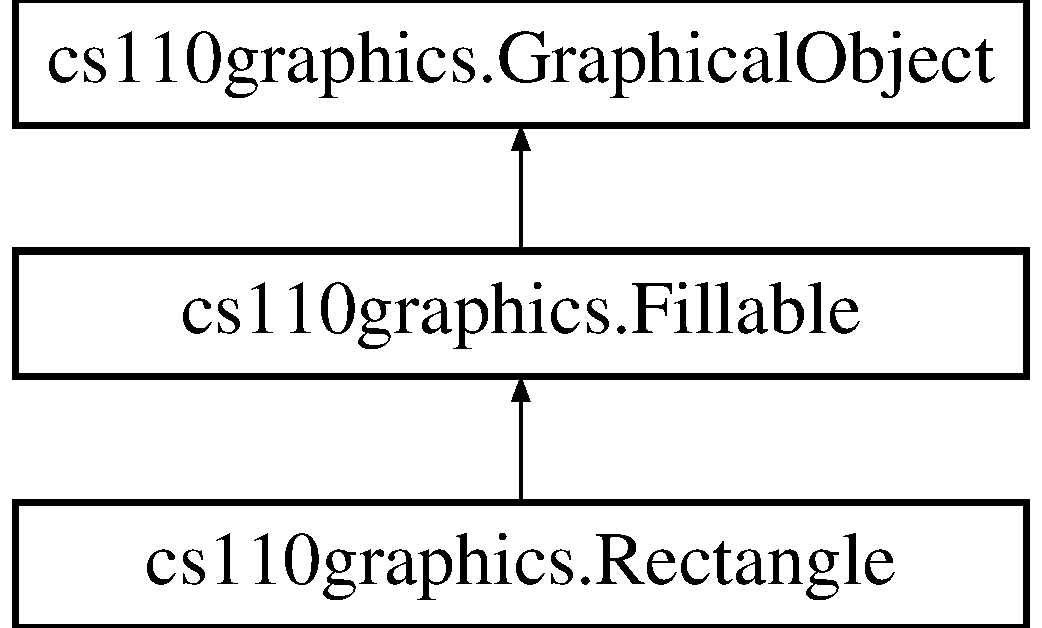
\includegraphics[height=3cm]{classcs110graphics_1_1Rectangle}
\end{center}
\end{figure}
\subsection*{Public Member Functions}
\begin{DoxyCompactItemize}
\item 
\hypertarget{classcs110graphics_1_1Rectangle_a57049aac9a7f4aa8823112290888a6a8}{
def {\bfseries \_\-\_\-init\_\-\_\-}}
\label{classcs110graphics_1_1Rectangle_a57049aac9a7f4aa8823112290888a6a8}

\item 
def \hyperlink{classcs110graphics_1_1Rectangle_a080e6851b24278d7533e0fa9920ea036}{set\_\-side\_\-lengths}
\begin{DoxyCompactList}\small\item\em Sets the width and height of the \hyperlink{classcs110graphics_1_1Rectangle}{Rectangle}. \item\end{DoxyCompactList}\end{DoxyCompactItemize}


\subsection{Detailed Description}
A rectangle, which can be added to a \hyperlink{classcs110graphics_1_1Window}{Window} object. Required Parameters:
\begin{DoxyItemize}
\item window -\/ \hyperlink{classcs110graphics_1_1Window}{Window} -\/ the window which the object will be added to.
\end{DoxyItemize}

Optional Parameters:
\begin{DoxyItemize}
\item width -\/ int -\/ sets the width of the \hyperlink{classcs110graphics_1_1Square}{Square}. (default: 40)
\item height -\/ int -\/ sets the height of the \hyperlink{classcs110graphics_1_1Square}{Square}. (default: 40)
\item center -\/ tuple -\/ sets the center of the \hyperlink{classcs110graphics_1_1Square}{Square}. (default: (200, 200)) 
\end{DoxyItemize}

\subsection{Member Function Documentation}
\hypertarget{classcs110graphics_1_1Rectangle_a080e6851b24278d7533e0fa9920ea036}{
\index{cs110graphics::Rectangle@{cs110graphics::Rectangle}!set\_\-side\_\-lengths@{set\_\-side\_\-lengths}}
\index{set\_\-side\_\-lengths@{set\_\-side\_\-lengths}!cs110graphics::Rectangle@{cs110graphics::Rectangle}}
\subsubsection[{set\_\-side\_\-lengths}]{\setlength{\rightskip}{0pt plus 5cm}def cs110graphics.Rectangle.set\_\-side\_\-lengths ( {\em self}, \/   {\em width}, \/   {\em height})}}
\label{classcs110graphics_1_1Rectangle_a080e6851b24278d7533e0fa9920ea036}


Sets the width and height of the \hyperlink{classcs110graphics_1_1Rectangle}{Rectangle}. 

The documentation for this class was generated from the following file:\begin{DoxyCompactItemize}
\item 
cs110graphics.py\end{DoxyCompactItemize}

\hypertarget{classcs110graphics_1_1Square}{
\section{cs110graphics.Square Class Reference}
\label{classcs110graphics_1_1Square}\index{cs110graphics::Square@{cs110graphics::Square}}
}


A square, which can be added to a \hyperlink{classcs110graphics_1_1Window}{Window} object.  
Inheritance diagram for cs110graphics.Square::\begin{figure}[H]
\begin{center}
\leavevmode
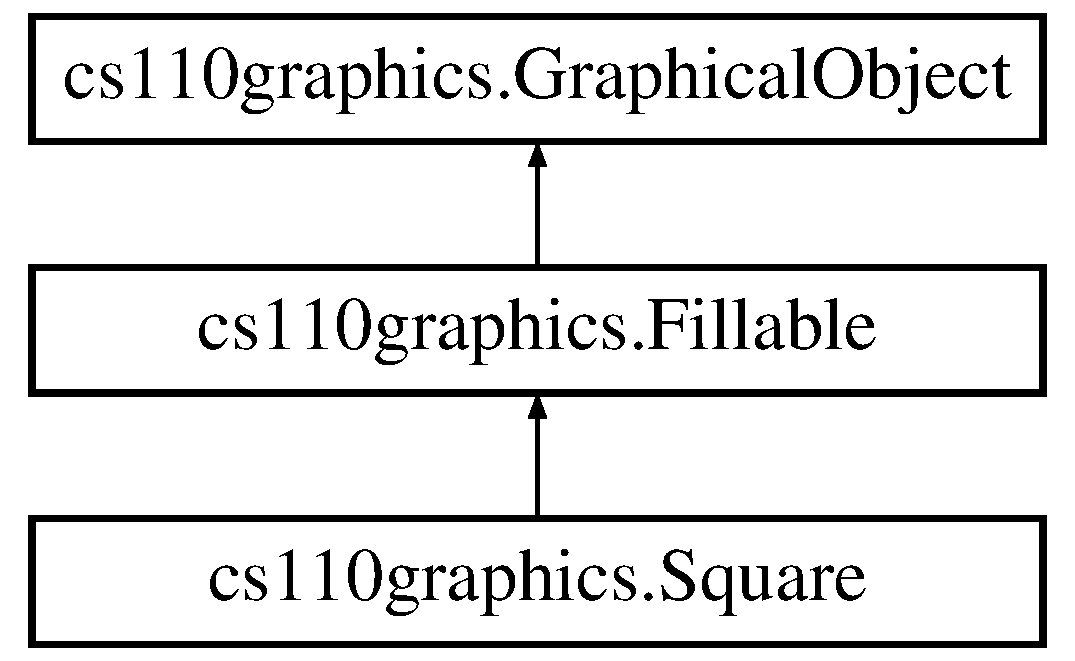
\includegraphics[height=3cm]{classcs110graphics_1_1Square}
\end{center}
\end{figure}
\subsection*{Public Member Functions}
\begin{DoxyCompactItemize}
\item 
\hypertarget{classcs110graphics_1_1Square_ae4b847029070a73478fd7dd2eefeb58e}{
def {\bfseries \_\-\_\-init\_\-\_\-}}
\label{classcs110graphics_1_1Square_ae4b847029070a73478fd7dd2eefeb58e}

\item 
def \hyperlink{classcs110graphics_1_1Square_a4b650f9ef28d4fab88d36ce65e8e0cf1}{set\_\-side\_\-length}
\begin{DoxyCompactList}\small\item\em Sets the side length of the \hyperlink{classcs110graphics_1_1Square}{Square}. \item\end{DoxyCompactList}\end{DoxyCompactItemize}


\subsection{Detailed Description}
A square, which can be added to a \hyperlink{classcs110graphics_1_1Window}{Window} object. Required Parameters:
\begin{DoxyItemize}
\item window -\/ \hyperlink{classcs110graphics_1_1Window}{Window} -\/ the window which the object will be added to.
\end{DoxyItemize}

Optional Parameters:
\begin{DoxyItemize}
\item side\_\-length -\/ int -\/ sets the side length of the \hyperlink{classcs110graphics_1_1Square}{Square}. (default: 40)
\item center -\/ tuple -\/ sets the center of the \hyperlink{classcs110graphics_1_1Square}{Square}. (default: (200, 200)) 
\end{DoxyItemize}

\subsection{Member Function Documentation}
\hypertarget{classcs110graphics_1_1Square_a4b650f9ef28d4fab88d36ce65e8e0cf1}{
\index{cs110graphics::Square@{cs110graphics::Square}!set\_\-side\_\-length@{set\_\-side\_\-length}}
\index{set\_\-side\_\-length@{set\_\-side\_\-length}!cs110graphics::Square@{cs110graphics::Square}}
\subsubsection[{set\_\-side\_\-length}]{\setlength{\rightskip}{0pt plus 5cm}def cs110graphics.Square.set\_\-side\_\-length ( {\em self}, \/   {\em side\_\-length})}}
\label{classcs110graphics_1_1Square_a4b650f9ef28d4fab88d36ce65e8e0cf1}


Sets the side length of the \hyperlink{classcs110graphics_1_1Square}{Square}. 

The documentation for this class was generated from the following file:\begin{DoxyCompactItemize}
\item 
cs110graphics.py\end{DoxyCompactItemize}

\hypertarget{classcs110graphics_1_1Text}{
\section{cs110graphics.Text Class Reference}
\label{classcs110graphics_1_1Text}\index{cs110graphics::Text@{cs110graphics::Text}}
}


\hyperlink{classcs110graphics_1_1Text}{Text} which can be added to a \hyperlink{classcs110graphics_1_1Window}{Window} object.  
Inheritance diagram for cs110graphics.Text::\begin{figure}[H]
\begin{center}
\leavevmode
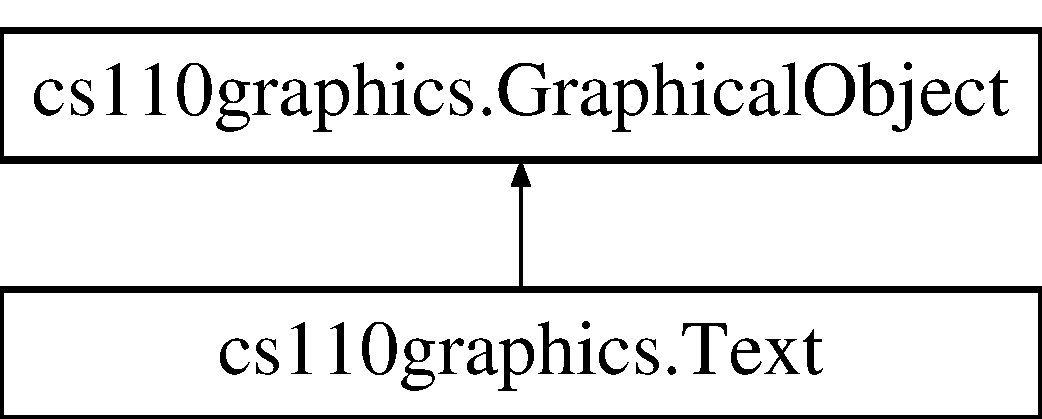
\includegraphics[height=2cm]{classcs110graphics_1_1Text}
\end{center}
\end{figure}
\subsection*{Public Member Functions}
\begin{DoxyCompactItemize}
\item 
\hypertarget{classcs110graphics_1_1Text_a022ce78a2945edbd8dfe3c4498769a62}{
def {\bfseries \_\-\_\-init\_\-\_\-}}
\label{classcs110graphics_1_1Text_a022ce78a2945edbd8dfe3c4498769a62}

\item 
def \hyperlink{classcs110graphics_1_1Text_a6bd6f174fc82f2225a4d162ca6b90ec2}{move}
\begin{DoxyCompactList}\small\item\em Moves a graphical object dx pixels horizontally and dy pixels vertically. \item\end{DoxyCompactList}\item 
def \hyperlink{classcs110graphics_1_1Text_a615a76c8d2edd6c6af5d39d4e2577a27}{move\_\-to}
\begin{DoxyCompactList}\small\item\em Moves a graphical object to a point. \item\end{DoxyCompactList}\item 
def \hyperlink{classcs110graphics_1_1Text_ad470aa26235fc2f5f1459c3750251207}{set\_\-size}
\begin{DoxyCompactList}\small\item\em Sets the point size of the text. \item\end{DoxyCompactList}\item 
def \hyperlink{classcs110graphics_1_1Text_ab12aa7478ca6a2b2015b7e8544674c73}{set\_\-text}
\begin{DoxyCompactList}\small\item\em Sets the text. \item\end{DoxyCompactList}\end{DoxyCompactItemize}


\subsection{Detailed Description}
\hyperlink{classcs110graphics_1_1Text}{Text} which can be added to a \hyperlink{classcs110graphics_1_1Window}{Window} object. Required Parameters:
\begin{DoxyItemize}
\item window -\/ \hyperlink{classcs110graphics_1_1Window}{Window} -\/ the window which the object will be added to.
\item text -\/ str -\/ The text which is displayed.
\end{DoxyItemize}

Optional Parameters:
\begin{DoxyItemize}
\item center -\/ tuple of int $\ast$ int -\/ sets the center of the \hyperlink{classcs110graphics_1_1Image}{Image}. (default: (200, 200))
\item width -\/ int -\/ sets the size of the text. (default: 12) 
\end{DoxyItemize}

\subsection{Member Function Documentation}
\hypertarget{classcs110graphics_1_1Text_a6bd6f174fc82f2225a4d162ca6b90ec2}{
\index{cs110graphics::Text@{cs110graphics::Text}!move@{move}}
\index{move@{move}!cs110graphics::Text@{cs110graphics::Text}}
\subsubsection[{move}]{\setlength{\rightskip}{0pt plus 5cm}def cs110graphics.Text.move ( {\em self}, \/   {\em dx}, \/   {\em dy})}}
\label{classcs110graphics_1_1Text_a6bd6f174fc82f2225a4d162ca6b90ec2}


Moves a graphical object dx pixels horizontally and dy pixels vertically. Required Parameters:
\begin{DoxyItemize}
\item dx -\/ int
\item dy -\/ int 
\end{DoxyItemize}

Reimplemented from \hyperlink{classcs110graphics_1_1GraphicalObject_aa64d270fb83efa4a54e1a7953512f9cd}{cs110graphics.GraphicalObject}.\hypertarget{classcs110graphics_1_1Text_a615a76c8d2edd6c6af5d39d4e2577a27}{
\index{cs110graphics::Text@{cs110graphics::Text}!move\_\-to@{move\_\-to}}
\index{move\_\-to@{move\_\-to}!cs110graphics::Text@{cs110graphics::Text}}
\subsubsection[{move\_\-to}]{\setlength{\rightskip}{0pt plus 5cm}def cs110graphics.Text.move\_\-to ( {\em self}, \/   {\em point})}}
\label{classcs110graphics_1_1Text_a615a76c8d2edd6c6af5d39d4e2577a27}


Moves a graphical object to a point. Required Parameters:
\begin{DoxyItemize}
\item point -\/ tuple of (int $\ast$ int) 
\end{DoxyItemize}

Reimplemented from \hyperlink{classcs110graphics_1_1GraphicalObject_abe2d480265df7ac9447205c52c6946df}{cs110graphics.GraphicalObject}.\hypertarget{classcs110graphics_1_1Text_ad470aa26235fc2f5f1459c3750251207}{
\index{cs110graphics::Text@{cs110graphics::Text}!set\_\-size@{set\_\-size}}
\index{set\_\-size@{set\_\-size}!cs110graphics::Text@{cs110graphics::Text}}
\subsubsection[{set\_\-size}]{\setlength{\rightskip}{0pt plus 5cm}def cs110graphics.Text.set\_\-size ( {\em self}, \/   {\em size})}}
\label{classcs110graphics_1_1Text_ad470aa26235fc2f5f1459c3750251207}


Sets the point size of the text. Required Parameters:
\begin{DoxyItemize}
\item size -\/ int 
\end{DoxyItemize}\hypertarget{classcs110graphics_1_1Text_ab12aa7478ca6a2b2015b7e8544674c73}{
\index{cs110graphics::Text@{cs110graphics::Text}!set\_\-text@{set\_\-text}}
\index{set\_\-text@{set\_\-text}!cs110graphics::Text@{cs110graphics::Text}}
\subsubsection[{set\_\-text}]{\setlength{\rightskip}{0pt plus 5cm}def cs110graphics.Text.set\_\-text ( {\em self}, \/   {\em text})}}
\label{classcs110graphics_1_1Text_ab12aa7478ca6a2b2015b7e8544674c73}


Sets the text. Required Parameters:
\begin{DoxyItemize}
\item text -\/ string 
\end{DoxyItemize}

The documentation for this class was generated from the following file:\begin{DoxyCompactItemize}
\item 
cs110graphics.py\end{DoxyCompactItemize}

\hypertarget{classcs110graphics_1_1Timer}{
\section{cs110graphics.Timer Class Reference}
\label{classcs110graphics_1_1Timer}\index{cs110graphics::Timer@{cs110graphics::Timer}}
}


A class which continually runs a function after a delay.  
\subsection*{Public Member Functions}
\begin{DoxyCompactItemize}
\item 
\hypertarget{classcs110graphics_1_1Timer_a7d40cc83eb4083d4afd97c3ce5279e1a}{
def {\bfseries \_\-\_\-init\_\-\_\-}}
\label{classcs110graphics_1_1Timer_a7d40cc83eb4083d4afd97c3ce5279e1a}

\item 
def \hyperlink{classcs110graphics_1_1Timer_aba0aae9c8bfff7c626112f0020383a8d}{set\_\-function}
\begin{DoxyCompactList}\small\item\em Sets the function which is going to be run. \item\end{DoxyCompactList}\item 
def \hyperlink{classcs110graphics_1_1Timer_ae176b030095b0d96fa0e91f2c398c40a}{set\_\-interval}
\begin{DoxyCompactList}\small\item\em Sets the interval between executions of the function. \item\end{DoxyCompactList}\item 
def \hyperlink{classcs110graphics_1_1Timer_afe14c3fd66571d0186a54a4075f31b7e}{start}
\begin{DoxyCompactList}\small\item\em Starts the timer. \item\end{DoxyCompactList}\item 
def \hyperlink{classcs110graphics_1_1Timer_a26ae5eb7c7da929f7e2b6e17e4b709b1}{stop}
\begin{DoxyCompactList}\small\item\em Stops the timer. \item\end{DoxyCompactList}\end{DoxyCompactItemize}


\subsection{Detailed Description}
A class which continually runs a function after a delay. Required Parameters:
\begin{DoxyItemize}
\item window -\/ \hyperlink{classcs110graphics_1_1Window}{Window} -\/ the window which the timer will use to start and stop the animation.
\item interval -\/ int -\/ the time (in milliseconds) that the function will refresh.
\item func -\/ function -\/ the function which will be run. 
\end{DoxyItemize}

\subsection{Member Function Documentation}
\hypertarget{classcs110graphics_1_1Timer_aba0aae9c8bfff7c626112f0020383a8d}{
\index{cs110graphics::Timer@{cs110graphics::Timer}!set\_\-function@{set\_\-function}}
\index{set\_\-function@{set\_\-function}!cs110graphics::Timer@{cs110graphics::Timer}}
\subsubsection[{set\_\-function}]{\setlength{\rightskip}{0pt plus 5cm}def cs110graphics.Timer.set\_\-function ( {\em self}, \/   {\em func})}}
\label{classcs110graphics_1_1Timer_aba0aae9c8bfff7c626112f0020383a8d}


Sets the function which is going to be run. Required Parameters:
\begin{DoxyItemize}
\item func -\/ function 
\end{DoxyItemize}\hypertarget{classcs110graphics_1_1Timer_ae176b030095b0d96fa0e91f2c398c40a}{
\index{cs110graphics::Timer@{cs110graphics::Timer}!set\_\-interval@{set\_\-interval}}
\index{set\_\-interval@{set\_\-interval}!cs110graphics::Timer@{cs110graphics::Timer}}
\subsubsection[{set\_\-interval}]{\setlength{\rightskip}{0pt plus 5cm}def cs110graphics.Timer.set\_\-interval ( {\em self}, \/   {\em interval})}}
\label{classcs110graphics_1_1Timer_ae176b030095b0d96fa0e91f2c398c40a}


Sets the interval between executions of the function. Required Parameters:
\begin{DoxyItemize}
\item interval -\/ int 
\end{DoxyItemize}\hypertarget{classcs110graphics_1_1Timer_afe14c3fd66571d0186a54a4075f31b7e}{
\index{cs110graphics::Timer@{cs110graphics::Timer}!start@{start}}
\index{start@{start}!cs110graphics::Timer@{cs110graphics::Timer}}
\subsubsection[{start}]{\setlength{\rightskip}{0pt plus 5cm}def cs110graphics.Timer.start ( {\em self})}}
\label{classcs110graphics_1_1Timer_afe14c3fd66571d0186a54a4075f31b7e}


Starts the timer. \hypertarget{classcs110graphics_1_1Timer_a26ae5eb7c7da929f7e2b6e17e4b709b1}{
\index{cs110graphics::Timer@{cs110graphics::Timer}!stop@{stop}}
\index{stop@{stop}!cs110graphics::Timer@{cs110graphics::Timer}}
\subsubsection[{stop}]{\setlength{\rightskip}{0pt plus 5cm}def cs110graphics.Timer.stop ( {\em self})}}
\label{classcs110graphics_1_1Timer_a26ae5eb7c7da929f7e2b6e17e4b709b1}


Stops the timer. 

The documentation for this class was generated from the following file:\begin{DoxyCompactItemize}
\item 
cs110graphics.py\end{DoxyCompactItemize}

\hypertarget{classcs110graphics_1_1Window}{
\section{cs110graphics.Window Class Reference}
\label{classcs110graphics_1_1Window}\index{cs110graphics::Window@{cs110graphics::Window}}
}


This window acts as a canvas which other objects can be put onto.  
\subsection*{Public Member Functions}
\begin{DoxyCompactItemize}
\item 
\hypertarget{classcs110graphics_1_1Window_af926549e3d731847886302fa390f2863}{
def {\bfseries \_\-\_\-init\_\-\_\-}}
\label{classcs110graphics_1_1Window_af926549e3d731847886302fa390f2863}

\item 
def \hyperlink{classcs110graphics_1_1Window_a34064de02d5149841a23764e78085d18}{add}
\begin{DoxyCompactList}\small\item\em Adds an object of type \hyperlink{classcs110graphics_1_1GraphicalObject}{GraphicalObject} to the \hyperlink{classcs110graphics_1_1Window}{Window} object. \item\end{DoxyCompactList}\item 
def \hyperlink{classcs110graphics_1_1Window_a14aba875d32f8a70a0c5a80ac3f18a92}{remove}
\begin{DoxyCompactList}\small\item\em Removes an object of type \hyperlink{classcs110graphics_1_1GraphicalObject}{GraphicalObject} to the \hyperlink{classcs110graphics_1_1Window}{Window} object, assuming the object being deleted exists. \item\end{DoxyCompactList}\item 
def \hyperlink{classcs110graphics_1_1Window_a981a3115f1f22099549117313f38333c}{set\_\-background}
\begin{DoxyCompactList}\small\item\em Sets the background color of the canvas. \item\end{DoxyCompactList}\item 
def \hyperlink{classcs110graphics_1_1Window_a9b548549f8f09ca3f29e6e80483e21d2}{set\_\-height}
\begin{DoxyCompactList}\small\item\em Sets the height of the canvas. \item\end{DoxyCompactList}\item 
def \hyperlink{classcs110graphics_1_1Window_a227c806c2acbcaca9958ba3b610a85f6}{set\_\-title}
\begin{DoxyCompactList}\small\item\em Sets the title of the window holding the canvas. \item\end{DoxyCompactList}\item 
def \hyperlink{classcs110graphics_1_1Window_a55036373bfb4437eb4368a39fedb8722}{set\_\-width}
\begin{DoxyCompactList}\small\item\em Sets the width of the canvas. \item\end{DoxyCompactList}\end{DoxyCompactItemize}


\subsection{Detailed Description}
This window acts as a canvas which other objects can be put onto. Required Parameters:
\begin{DoxyItemize}
\item width -\/ int -\/ Width of canvas.
\item height -\/ int -\/ Height of canvas.
\item background -\/ str -\/ Background color of canvas. Can be either the name of a color (\char`\"{}yellow\char`\"{}), or a hex code (\char`\"{}\#FFFF00\char`\"{}).
\item name -\/ str -\/ The title of the window.
\item first\_\-function -\/ proc(Window) -\/ When the window is created, it runs this function after everything is run. (default: None)
\item master -\/ unknown type -\/ necessary for the creation of the Tkinter widgets. (default: None) 
\end{DoxyItemize}

\subsection{Member Function Documentation}
\hypertarget{classcs110graphics_1_1Window_a34064de02d5149841a23764e78085d18}{
\index{cs110graphics::Window@{cs110graphics::Window}!add@{add}}
\index{add@{add}!cs110graphics::Window@{cs110graphics::Window}}
\subsubsection[{add}]{\setlength{\rightskip}{0pt plus 5cm}def cs110graphics.Window.add ( {\em self}, \/   {\em graphic})}}
\label{classcs110graphics_1_1Window_a34064de02d5149841a23764e78085d18}


Adds an object of type \hyperlink{classcs110graphics_1_1GraphicalObject}{GraphicalObject} to the \hyperlink{classcs110graphics_1_1Window}{Window} object. Required Parameters:
\begin{DoxyItemize}
\item graphic -\/ \hyperlink{classcs110graphics_1_1GraphicalObject}{GraphicalObject} 
\end{DoxyItemize}\hypertarget{classcs110graphics_1_1Window_a14aba875d32f8a70a0c5a80ac3f18a92}{
\index{cs110graphics::Window@{cs110graphics::Window}!remove@{remove}}
\index{remove@{remove}!cs110graphics::Window@{cs110graphics::Window}}
\subsubsection[{remove}]{\setlength{\rightskip}{0pt plus 5cm}def cs110graphics.Window.remove ( {\em self}, \/   {\em graphic})}}
\label{classcs110graphics_1_1Window_a14aba875d32f8a70a0c5a80ac3f18a92}


Removes an object of type \hyperlink{classcs110graphics_1_1GraphicalObject}{GraphicalObject} to the \hyperlink{classcs110graphics_1_1Window}{Window} object, assuming the object being deleted exists. Required Parameters:
\begin{DoxyItemize}
\item graphic -\/ \hyperlink{classcs110graphics_1_1GraphicalObject}{GraphicalObject} 
\end{DoxyItemize}\hypertarget{classcs110graphics_1_1Window_a981a3115f1f22099549117313f38333c}{
\index{cs110graphics::Window@{cs110graphics::Window}!set\_\-background@{set\_\-background}}
\index{set\_\-background@{set\_\-background}!cs110graphics::Window@{cs110graphics::Window}}
\subsubsection[{set\_\-background}]{\setlength{\rightskip}{0pt plus 5cm}def cs110graphics.Window.set\_\-background ( {\em self}, \/   {\em background})}}
\label{classcs110graphics_1_1Window_a981a3115f1f22099549117313f38333c}


Sets the background color of the canvas. Required Parameters:
\begin{DoxyItemize}
\item background -\/ string 
\end{DoxyItemize}\hypertarget{classcs110graphics_1_1Window_a9b548549f8f09ca3f29e6e80483e21d2}{
\index{cs110graphics::Window@{cs110graphics::Window}!set\_\-height@{set\_\-height}}
\index{set\_\-height@{set\_\-height}!cs110graphics::Window@{cs110graphics::Window}}
\subsubsection[{set\_\-height}]{\setlength{\rightskip}{0pt plus 5cm}def cs110graphics.Window.set\_\-height ( {\em self}, \/   {\em height})}}
\label{classcs110graphics_1_1Window_a9b548549f8f09ca3f29e6e80483e21d2}


Sets the height of the canvas. Required Parameters:
\begin{DoxyItemize}
\item height -\/ int 
\end{DoxyItemize}\hypertarget{classcs110graphics_1_1Window_a227c806c2acbcaca9958ba3b610a85f6}{
\index{cs110graphics::Window@{cs110graphics::Window}!set\_\-title@{set\_\-title}}
\index{set\_\-title@{set\_\-title}!cs110graphics::Window@{cs110graphics::Window}}
\subsubsection[{set\_\-title}]{\setlength{\rightskip}{0pt plus 5cm}def cs110graphics.Window.set\_\-title ( {\em self}, \/   {\em name})}}
\label{classcs110graphics_1_1Window_a227c806c2acbcaca9958ba3b610a85f6}


Sets the title of the window holding the canvas. Required Parameters:
\begin{DoxyItemize}
\item name -\/ string 
\end{DoxyItemize}\hypertarget{classcs110graphics_1_1Window_a55036373bfb4437eb4368a39fedb8722}{
\index{cs110graphics::Window@{cs110graphics::Window}!set\_\-width@{set\_\-width}}
\index{set\_\-width@{set\_\-width}!cs110graphics::Window@{cs110graphics::Window}}
\subsubsection[{set\_\-width}]{\setlength{\rightskip}{0pt plus 5cm}def cs110graphics.Window.set\_\-width ( {\em self}, \/   {\em width})}}
\label{classcs110graphics_1_1Window_a55036373bfb4437eb4368a39fedb8722}


Sets the width of the canvas. Required Parameters:
\begin{DoxyItemize}
\item width -\/ height 
\end{DoxyItemize}

The documentation for this class was generated from the following file:\begin{DoxyCompactItemize}
\item 
cs110graphics.py\end{DoxyCompactItemize}

\printindex
\end{document}
